%
% METU Institute of Natural and Applied Sciences Thesis example
%
% Edited and Commented by Utku Erdoğdu 2012
% Updated by Ahmet KARA 2013
%
% Please read the explanations so that you can customize the document
%
% Files needed by this document:
% metu.cls
% metu11.def (if you will use 11pt fonts)
% metu12.def (if you will use 12pt fonts)
% metu10.def (if you will use 10pt fonts)
%
% Possible Options Here:
%
% oneandhalf, double, single : Line spacing used in the thesis. Default and institute preference is
% single.
%
% 10pt, 11pt, 12pt : Font size Default is 10pt, which is institue choice.
%
% pntr, pntc, pnbt : Page number position. Options are top center, top right or bottom. Default and
% institute preference is page numbers at bottom. When page numbers are at the top bottom margins
% are skewed.
%
% chaproman, chaparabic: Chapter numbering format. Options are roman numbers and arabic numbers.
% Default is roman, institute prefers arabic
%
% oneside, twoside : Printing style. Default is twoside, which is institute choice. In this style
% chapters begin from odd numbered pages.
%
% tr, eng : Document language. This is useful if you want to translate your thesis into
% Turkish. Then you give the option tr and use \ifturkish. . .\else. . .\fi  whenever you want
% to do something only for Turkish or only for English. Default is eng.
% IMPORTANT!! : For official institute documents you should not use this option.
% The Turkish format is only supplied for custom translations.
%
% ceng,aee,arme.. : You can use the abbreviated form of your department here and there is no further need to
% define the department name below. If your department name is not among the below list of defined
% departments, you should use \department and \turkishdepartment macros to define the name of your
% department.
%
% Defined Departments and Abbreviations:
% --------------------------------------
% Computer Engineering : ceng
% Aerospace Engineering : aee
% Archaeometry : arme
% Architecture : arch
% Biochemistry : bch
% Biology : biol
% Biomedical Engineering : bme
% Biotechnology : btec
% Building Science : bs
% Cement Engineering : ceme
% Chemical Engineering : che
% Chemistry : chem
% City and Regional Planning : crp
% City Planning : cp
% Civil Engineering : ce
% Computational Design and Fabrication Technologies in Architecture : arcd
% Computer Education and Instructional Technology : cte
% Design Research for Interaction : iddi
% Earthquake Studies : eqs
% Earth System Science : ess
% Electrical and Electronics Engineering : ee
% Engineering Management : em
% Engineering Sciences : es
% Environmental Engineering : enve
% Food Engineering : fde
% Geodetics - Geographical Information Technologies : ggit
% Geological Engineering : geoe
% Hydrosystems Engineering : he
% Industrial Design : id
% Industrial Engineering : ie
% Mathematics : math
% Mechanical Engineering : mech
% Metallurgical and Materials Engineering : mete
% Micro and Nanotechnology : mnt
% Mining Engineering : mine
% Operational Research : or
% Petroleum and Natural Gas Engineering : pete
% Physics : phys
% Polymer Science and Technology : pst
% Regional Planning : rp
% Restoration : rest
% Secondary Science and Mathematics Education : ssme
% Software Engineering : se
% Statistics : stat
% Structural Mechanics : st
%
% phd, ms : Degree Received. Ph.D. or M.S. Default is M.S.
%
% End of Options
%\documentclass[10pt,single,chaparabic,ceng,phd,eng]{metu}
\documentclass[12pt,oneandhalf,chaparabic,phys,ms,eng]{metu}
% You can delete next line If your thesis does not have an appendix
\usepackage{appendix}


%
% Use your latex packages here
\usepackage{graphicx} %grapik eklemek için gerekli-latex->pdf şeklinde compile edersek .jpeg 
%formatında ekleme yapabiliyoruz.
\usepackage{afterpage}

% End of Latex Packages
%
% Any personal Latex definition, decleration, etc.


% End of personal stuff
%
% Personal Information
% ----------------------------
%
% Please check this part and fill in information about your thesis
%
% Name and Surname
\author{Ece Aşılar}
% Updated by Ece ASILAR
% Thesis Title English and Turkish
\title{Search for Pair Production of a Heavy Quark Decaying into top quark and photon in Semi-leptonic Channel with the CMS Detector in the LHC}
\turkishtitle{LHC'DE CMS DENEYiNDE TOP KUARK VE FOTONA BOZUNAN YENİ AĞIR KUARKIN YARI LEPTONIK KANALDA ÇIFT URETILMESININ ARAŞTIRILMASI }
% Department : English and Turkish
%
% Some of the departments are pre-defined, you need not redeclare them. You can use them by just
% giving an option to \documentclass. See documentation for options above. If you will define your
% department here do not use ``Department'' or ``Bölümü'' words.
%\department{Physics Department}
%\turkishdepartment{Fizik Bölümü}
%
%
% Date : You should indicate the month of your thesis defence in English.
% Default is this month
%
\date{July 2014}
%
% Approval Page Details
% --------------------------
% For each command you can give the title as optional parameter enclosed in [ ]
% This also handles the Turkish titles if you're planning to produce Turkish version of the
% document. If you'll hard code the title, you need to use turkish version of each command after
% the command itself
%
% prof : Prof. Dr.
% assocprof : Assoc. Prof. Dr.
% assistprof : Assist. Prof. Dr.
% dr : Dr.
%
% Director of Institute
\director[prof]{Canan Özgen}
% Head of Department
\headofdept[prof]{Mehmet Zeyrek }
%
% Supervisor : English and Turkish
\supervisor[prof]{Ali Murat Güler}
% \turkishsupervisor{  } %if you will hard-code the academic title
%
% Affiliation of Supervisor in English and possibly in Turkish
\departmentofsupervisor{Physics Department, METU}
% Co Supervisor if Any : English and Turkish
% You can just delete the next line if you don't have a co-supervisor
%\cosupervisor[prof]{Reda Alhajj}
% \turkishcosupervisor{Prof. Dr. Reda Alhajj} %if you will hard-code the academic title
% Affiliation of Co-Supervisor
% You can just delete the next line if you don't have a co-supervisor
%\departmentofcosupervisor{Computer Science Dept., Univ. of Calgary}
%
% Committee Members
% In general members are sorted according to their academic titles
%
% Proffesors (1)
% Associate Professors (2)
% Assistant Professors (3)
% Other (4)
%
% IMPORTANT:  All affiliatons should fit in a single line
% If affiliation line is broken into two lines you should shorten the affiliation by using
% abbrevations or any other means
%
% First committee member should be the chair of examining committee
% Typically the chair is one of the highest ranked committee members
% Ask your supervisor if you are not sure
\committeememberi[prof]{Ramazan Sever}
\affiliationi{Physics Department, METU}
% Second committee member is always your supervisor
\committeememberii[prof]{Ali Murat Güler}
\affiliationii{Physics Department, METU}
% If you are an M.Sc. student and your Co-Supervisor is in your
% examination committee, then third committee member is always your co-supervisor
%
% IMPORTANT: If you are Ph.D. student your co-supervisor can not be in your
% examination committee.
\committeememberiii[prof]{Orhan Çakır}
\affiliationiii{Physics Department, AU}
% Fourth committee member
\committeememberiv[prof]{Altuğ Özpineci}
\affiliationiv{Physics Department, METU}
% Fifth committee member
\committeememberv[prof]{Osman Yılmaz}
\affiliationv{Physics Department, METU}
%

% Keywords : English & Turkish, Comma seperated
\keywords{LHC,
CMS,
Heavy Quark,
Extra Dimentions,
Randall Sundrum Model,
Warped Geometry
}
\anahtarklm{BHC,
CMS,
Ağır Kuark
Extra boyutlar,
Randall Sundrum Model,
Çarpık Uzay
}
%
% Abstract in English
%
\abstract{In this thesis, a search for a pair produced excited quark, $t^*$, which decays exclusively to a top quark and a photon, is performed by considering semi-leptonic decay channel. This entails that there are two isolated photons, at least 4 well-reconstructed jets and one lepton, which can be either a single isolated muon or electron, in the final state. Moreover, the chi-square  sorting method and matrix method is presented to reconstruct signal and to determine fake rate of photons coming from leptons and jets, for background reconstruction, respectively. Tag and Probe method and QCD-enriched samples are also implied to make use of matrix method. In this study, proton-proton collision data collected by CMS at 8 TeV corresponding to an integrated luminosity of 19.6${fb}^{-1}$ is investigated. Analysis is performed in a model independent way while a heavy spin-3/2 excitation of a heavy spin-1/2 quark indicated by ”Rarita-Schwinger” vector spinor Lagrangian is the most favourable choice among other beyond the standard models. As a result of this study, no significant excess is observed over expectations and a lower limit is set on a t* quark mass of 969 ${GeV/c}^{2}$ at 95$\%$ confidence level.  }
%
% Turkish Abstract
%
\oz{Bu tezde LHC’de CMS deneyinde top ve foton rezonansı çalışıldı. Temel olarak kompozit top kuark üzerine yoğunlaşılırken analiz herhangi bir modele dayanmamaktadır. Çift olarak üretilen yeni ağır kuarkın top kuark ve fotona gittiği kanal yarı leptonik olarak çalışıldı.  Bu da son durumda 2 foton, 1 muon veya 1 elektron ve en az 4 iyi tespit edilmiş jetin varlığını gösterir. Kanal araştırılırken iki temel yöntem kullanıldı. Sinyal bölgesi saptaması için Chisquare elemesi kullanılırken ardalanın belirlenmesi için Matris metodu kullanıldı. Matris metodunda etiketle-ölç tekniği ve zenginleştirilmiş QCD veri örneği ile yapılan çalışmalar önemli rol oynadı. Bu araştırmada 19.6 ${fb}^{-1}$ toplam ışınlığa denk gelen 8 TeV çarpışma verisi incelenmiştir. Sonuç olarak, beklentilerin üzerinde bir sapma gözlenmemesinin yanında yeni ağır kuark kütlesine 95$\%$ güven seviyesinde 969 ${GeV/c}^{2}$ olarak bir alt sınır konuldu.
}
%
% Dedication
\dedication{\textit{To my mother and brother\\\vspace{1cm}Şenay Özçiftçi, Mehmetefe Aşılar}}
%
%
% Acknowledgements
\acknowledgments{
First of all, I would like to thank to my supervisor Prof. Ali Murat Güler for his continuous support and for giving me the great opportunity to work at CMS at CERN. \\
I would like to thank all my collaborators at CMS especially to Yeng-Ming Tzeng (Jacky), and Shin-Shan Yu (Eiko) for accepting me their group. I would also like to thank Marco Cardaci for his endless support during this search. I managed to develope a tag and probe code and calculate fake rate from leptons with his help. His logical thinking, patience and enthusiasm have been great motivative to me. He has been such a wonderful mentor to me. I like also to thank Yu-Hsian Chang and Kai-Feng Chen without them it would be impossible to finalize this search. \\
I would also like to thank the rest of my thesis examining committee: Prof. Dr. Orhan Çakır, Prof. Dr. Altuğ Özpineci, Prof. Dr. Ramazan Sever, Prof. Dr. Osman Yılmaz. \\
In addition, I like to thank Prof. Mithat Kaya and Özlem Kaya, Cemali Kılınç, Metin Yalvaç, Buğra Bilin for their friendship. \\
My sincere thanks also goes to Gokhan Alkaç for his many scientific advices and close friendship during my undergraduate and graduate education. \\
I am thankful to all my friends particularly Özlem Yavaş, Hakan Keskin and Zeynep Özer for their motivations and many helpful discussions. \\
Furthermore, I would like to thank my mother and brother for supporting me materially and spiritually throughout my life. \\
Finally, this thesis work is financially supported by Turkish Atomic Energy Agency with Project No: 05K120010.
 }
%
% End of Personal and Introductory Information
%%%%%%%%%%%%%%%%%%%%%%%%%%%%%%%%%5

%%% !!! This two should be last lines before \begin{document}, do no move them !!!
\usepackage[pdftex]{hyperref}
\usepackage[all]{hypcap}
\begin{document}
% Preliminaries
\begin{preliminaries}
% If you are willing to use any custom stuff before Chapters, put it here
% Such as List of Abbreviations
% Check the abbreviations.tex for a template list of abbreviations
%\begin{glossary}
%\end{glossary}
%\clearpage

%\newglossaryentry{domain-knowledge}{%
%  name={domain knowledge},%
%  description={valid knowledge used to refer to an area of human endeavour, an autonomous computer activity, or other specialized discipline}}

\newacronym{atlas}{ATLAS}{A Toroidal LHC Apparatus}
\newacronym{alice}{ALICE}{A Large Ion Collider Experiment}
\newacronym{sm}{SM}{Standard Model}
\newacronym{susy}{SUSY}{Supersymmetry}
\newacronym{bsm}{BSM}{Beyond the Standard Model}
\newacronym{cern}{CERN}{European Organization for Nuclear Research}
\newacronym{cm}{CM}{Center of Mass}
\newacronym{cms}{CMS}{Compact Muon Solenoid}
\newacronym{cmssw}{CMSSW}{CMS SoftWare framework}
\newacronym{daq}{DAQ}{Data Acquisition}
\newacronym{ecal}{ECAL}{Electromagnetic Calorimeter}
\newacronym{ewk}{EWK}{Electroweak Theory}
\newacronym{ewsb}{EWSB}{Electroweak Symmetry Breaking}
\newacronym{gut}{GUT}{Grand Unified Theory}
\newacronym{hcal}{HCAL}{Hadron Calorimeter}
\newacronym{hf}{HF}{Hadron Calorimeter (Forward)}
\newacronym{lhc}{LHC}{Large Hadron Collider}
\newacronym{lhcb}{LHCb}{the Large Hadron Collider Beauty Experiment}
\newacronym{linac}{LINAC}{Linear particle Accelerator}
\newacronym{pdg}{PDG}{Particle Data Group}
\newacronym{qed}{QED}{\textbf{quantum electrodynamics}}
\newacronym{gut}{GUT}{Grand Unified Theory}
\newacronym{qft}{QFT}{Quantum Field Theory}
\newacronym{qcd}{QCD}{\textbf{quantum chromodynamics}}
\newacronym{sms}{SMS}{Simplified Model Spectra}
\newacronym{vev}{VEV}{vacuum expectation value}
\newacronym{ssb}{SSB}{spontaneous breaking of the SM gauge symmetry}
\newacronym{dm}{DM}{Dark Matter}
\newacronym{cmb}{CMB}{cosmic Microwave Background}
\newacronym{lsp}{LSP}{lightest supersymmetric particle}
\newacronym{mssm}{MSSM}{minimal supersymmetric extension of the standard model}
\newacronym{cmssm}{cMSSM}{constrained MSSM}
\newacronym{pf}{PF}{particle flow}

%\begin{abbreviations}
%\noindent
%\begin{longtable}[l]{lp{10cm}}
%ALICE & A Large Ion Collider Experiment\\
%ATLAS & A Toroidal LHC Apparatus\\                 
%BSM   & Beyond the Standard Model\\
%CERN  & European Organization for Nuclear Research\\
%CM    & Center of Mass\\
%CMS   & Compact Muon Solenoid experiment\\
%CMSSW & CMS SoftWare framework\\
%DAQ   & Data Acquisition\\
%ECAL  & Electromagnetic Calorimeter\\
%EWK   & Electroweak Theory\\
%GUT   & Grand Unified Theory\\
%HCAL  & Hadron Calorimeter\\
%HF    & Hadron Calorimeter (Forward)\\
%LHC   & Large Hadron Collider\\
%LHCb  & the Large Hadron Collider Beauty Experiment\\
%LINAC & Linear particle Accelerator\\
%PDG   & Particle Data Group\\
%QED   & Quantum Electrodynamics\\
%QFT   & Quantum Field Theory\\
%SM    & Standard Model\\
%SMS   & Simplified Model Spectra\\
%SUSY  & Supersymmetry\\
%\end{longtable}

%\end{abbreviations}
%\begin{table}[ht]
%\begin{center}
%\begin{tabular}{cccc}
%\multicolumn{4}{ c }{List of Abbreviations}\\
%AA & blablabala & BB & Bla bla\\
%AA & blablabala & BB & Bla bla\\
%AA & blablabala & BB & Bla bla\\
%AA & blablabala & BB & Bla bla\\
%AA & blablabala & BB & Bla bla\\
%\end{tabular}
%\end{center}
%\end{table}
%
%
%



% End of Preliminaries
\end{preliminaries}
%
% Latex content Goes Here
%
%
%%%%%%%%%%%%%%%%%%%%%%%%%%%%%%%%%%%%%%%%%%%%%%%%%%%%%%%%%%%%
\chapter{Introduction}

This study puts into limelight the top quark and photon physics at CMS. The former, top quark was discovered as the sixth missing quark to complete the three generations of the Standard Model(SM), in 1994. Since then experimental precision has been advanced so that the top quark mass measured as 173.5 $\pm$ 0.6 $\pm$ 0.8 $GeV/ c^2$  (June 2012 PDG value) \cite{R24}.  Due to heaviness of top quark many models foresee that top quark is a composit particle rather than an elementary one \cite{R25,R29}. As for the latter, the photon is important because $\gamma$+jets and $\gamma$$\gamma$ processes are background to Higgs searches and searches beyond the standard model(BSM). Besides this, CMS dedector has a very comprehensive Electromagnetic calorimeter (ECAL) and therefore diphoton mass resolution is very precise, namely about 1$\%$ at 100 GeV.

Although SM has a proven success in describing the current data, it does not include the gravitation. The Randall-Sundrum(RS) \cite{R30,R31} Model solves the hierarchy problem between the electroweak and Planck scales by introducing extra-dimentions that gravity can penetrate. Thus, one possibility for $t^*$ is to be a spin-3/2 Regge excitation in RS model.
Moreover, since a resonance of $t$ + $\gamma$ has not been probed in CMS yet, it is essential to look for pair production of heavy quark decaying in to top quark and a photon semi-leptonically.

For this analysis, it is assumed that $t^*$$\rightarrow$$t$$+$$\gamma$ has a 100$\% $ branching fraction as it is dominant channel over  $t^*$$\rightarrow$$t+g$ and  $t^*$$\rightarrow$$t+Z$. Only pair production of $t^*$ is considered because it has a higher production cross section than single production of $t^*$ at the LHC. This is due to the fact that mixing between spin-3/2 and spin-1/2 states is suppressed \cite{R9}. Although a spin-3/2 RS resonance is focussed, the analysis is performed in a model independent way. The semi-leptonic decay channel of the system is taken under consideration, i.e. $t$$\rightarrow$$b$$W$ with $W$$\rightarrow$$q$$q$ on one side and $W$$\rightarrow$$\ell$$\nu$ on the otherside, where $\ell$ maybe either an electron or a muon.

Purpose of this search is to find $t^*$ particle in other words to measure excess of events consistent with $t^*$ pair production more than 3$\sigma$ to claim as a discovery. In case the particle couldn't be found, a lower limit on mass of $t^*$ would be determined.

This thesis is mainly divided in three parts. The first chapter, which is introduction, explains the theory behind this research. The following chapter is reserved for the experimental setup which is CMS detector and the LHC. The subsequent chapter, chapter three, is dedicated to analysis part which contains $\chi^{2}$ sorting method in order to reconstruct signal and matrix method to discribe background. At the end, forth chapter, conclusions will be discussed. 
 
\section{Theory}
\subsection{Standard Model}
Nowadays, the Standard Model (SM) (see \cite{R32} for a pedagogical introduction) is the most comprehensive model which discribes the subatomic particles and their interactions (Table \ref{SMPar}). In SM, there are two types of subatomic particles, fermions and bosons. Fermions have half integer spin and therefore they obey the  Pauli Exclusion Principle and they can not stay in the same quantum state simultaneously. This phenomenon is known as Fermi-Dirac statistics. In Table \ref{SMPar} one can see 12 fundemental particles which imply that they can not be subdivided into smaller particles. It should be noted that all visible matter in the universe is formed of these 12 particles. Moreover, these particles have partners which are particles with the same mass, but opposite electromagnetic charge, color and opposite component of the weak isospin. These pairs are called antiparticles.
On the other hand, bosons have an integer spin and obey the Bose–Einstein statistics which allows particles aggregation in the same state. According to SM, bosons are force carriers of corresponding interaction which is shown in the Table \ref{SMFor}. In the Table, interactions are written with respect to their strength.  The range of interaction is inverse proportional to mass of intermediate boson; However, due to self interaction of gluons strong force behaves differently. Gluons are mediating particles of Strong force and couple to color charge. The coupling strength of Strong force is decreasing with the increasing energy which is called "asymptotic freedom". Due to this phenomenon it is impossible to give enough energy to seperate a quark-antiquark pair without producing a new quark-antiquark pair. Following the strength order Electromagnetic interaction is the second. Photon is a massless boson which mediates Electromagnetic interactions. Charged particles, for example electrons and muons interact with photon. Weak interaction has two mediator bosons, $W^{\pm}$ and $Z$. It has very low range $(10^{-18} m)$ because of mediating bosons have large mass. In addition to these forces, there is Gravity in the universe; however SM does not include. It can be said that due to its very low strength Gravity does not play an important role in particle level. 

%%%%%%Table1%%%%

\begin{table}[!hbt]
\caption{Fundamental particles of the Standard Model. Q is the electric charge of the particle}
\label{SMPar}
\begin{center}
\begin{tabular}{l c c c c c} %\hline
		 & 1.Gen. & 2.Gen. & 3.Gen. & Q & Force\\ \hline
\\
 Leptons    & { $ \nu_{e} \choose e$ } & { $ \nu_{\mu} \choose \mu$ } & { $ \nu_{\tau} \choose \tau$ } & { $ 0 \choose 1$ } &{ $ weak \choose em,weak$ }  \\ %\hline
\\
	Quarks & { $u \choose d$ } & { $c \choose s$ } & { $ t \choose b$ } & { $ +2/3 \choose -1/3$ } & $em$, $weak$, $strong$ \\

\\ %\hline
\end{tabular}
\end{center}
\end{table}

%%%%%%%%%%%%%

%%%%%Table2%%%%%

\begin{table} [!hbt]
\caption{Except gravitation, all forces and their intermediate bosons are described by the Standard Model}
\label{SMFor}
\begin{center}
\begin{tabular}{l c c c c } %\hline
		 Interactions & Coupling with & Intermediate boson & Boson mass & Range(m)\\
&&&(in GeV)& \\ \hline
\\
 strong & color & 8 gluons(g) & 0 & $10^{-15}$ \\ 
electromag. & el.charge & photon($\gamma$) & 0 & $\infty$ \\
weak&weak charge&$W^\pm , Z^0$ & 80,90 & $10^{-18}$ \\
gravitation&mass&graviton(G)&0&$\infty$\\
\\ 
\end{tabular}
\end{center}
\end{table}

%%%%%%%%%%%%%%

SM is a relativistic quantum field theory invariant under the local gauge transformation group in Formula \ref{gauge}.
Where $SU(3)_{C} $ represents a symmetry group for strong interaction while $SU(2)_{L} \otimes U(1)_{Y}$ stands for the group describing the electroweak interactions. 
 
\begin{eqnarray}
\label{gauge}
% \nonumber to remove numbering (before each equation)
	SU(3)_{C} \otimes SU(2)_{L} \otimes U(1)_{Y}
\end{eqnarray}

In 1961, Glashow introduced that there are three conserved weak currents related to the generators of the weak isospin group $SU(3)_{C}$ and one to the weak hypercharge group $U(1)_{Y}$.  A combination of two $SU(2)_{L}$ currents identifies charged weak currents, while a mixing of the $SU(2)$ and $U(1)$ currents indicates the neutral weak and the electromagnetic currents. The weak hypercharge can be extracted from the Formula \ref{hyper} where $Q$ is the electric charge and $I_{3}$ is the third component of the weak isospin I.

\begin{eqnarray}
\label{hyper}
% \nonumber to remove numbering (before each equation)
	Y=2(Q-I_{3})
\end{eqnarray}

In the Table \ref{SMFor}, one can easily see that $W^\pm , Z^0$ bosons have masses in order to explain short range of weak interaction. However, If explicit mass terms are implemeted to SM then SM losses the gauge invariance and thus the renormalizability of the field theory. In this point Higgs mechanism takes care of this mass problem by introducing spontaneous symmetry breaking \cite{SM}.
In the Standard Model, when the Weak and Electromagnetic force is unified it results in three $W$ bosons and $B^0$ boson which are gauge bosons mediating electroweak interaction. However, these Gauge bosons can not be observed physically. Z and  $\gamma$ bosons can be formed by electroweak symmetry breaking, $B^0$ and $W^0$ mix with the help of weak angle. This relation can be seen from equation \ref{Zbos}. 

\begin{eqnarray}
\label{Zbos}
% \nonumber to remove numbering (before each equation)
	{ \gamma \choose Z } = { cos \theta_W  sin \theta_W \choose -sin \theta_W cos \theta_W  } { B^0 \choose W^0 }
\end{eqnarray}

Additionally, superposition of $W^1$ and $W^2$ gauge bosons gives $W^{\pm}$. This symmetry breaking also brings up the Higgs boson. In 2012, the CMS \cite{RSM1} and ATLAS \cite{RSM2} experiments at the LHC introduce a new boson discovery with consistent properties with predicted Higgs boson within SM. 

The SM is in a well consistency with current experimental data obtained from particle accelerator experiments. Considering this, SM still have some theoretical inadequacies that a fundamental theory should not involve them. The  hiararchy problem is one of the examples of these inadequacies.

%%%%%%%%%%%%%%%%%%%%%%%%%%%%%%%%%%%
\subsubsection{The hiararchy problem in SM}
There are two hierarchy problems of SM. The first one is the little hierarchy problem.  The problem is that Quantum Field Theory (QFT) correction terms of free higgs mass are almost equal to higgs mass itself. One of the candidate BSMs to solve this problem is the Little Higgs model \cite{R6}. The model professes that the problem can be solved by adding new particles. These loop contributions are quadratically divergent and they are mostly coming from the loops involving top quark. The problem concered in this thesis actually the large hierarchy problem of SM. This problem occurs due to a large energy difference between electroweak scale and Plank scale where electroweak scale is the scale at which the symmetry between electromagnetism and the electroweak interaction is broken and Plank scale associated with gravity \cite{R7}. In other words, the electroweak force is $10^{32}$ times stronger than gravity and SM can not explain this. The problem can be solved by RS Model \cite{R30,R31} by a string theory inspired context.
%%%%%%%%%%%%%%%%%%%%%%%%%%%%%%%%%%%

\subsection{The Randall-Sundrum Model}

Generally, it is supposed that the universe, we live in, has 3 spatial dimensions. However, it is not have to be like that. Extra spatial dimensions is introduced to unify four fundemental forces by Gunnar Nordström, in 1914. He asserted a five dimensional theory to combine electromagnetism and a scaler version of gravity.  The idea \cite{R33} was further detailed by Theodor Kaluza and Oscar Klein after the development of general relativity. Although the Kaluza-Klein theory was not succesfull in unifying all forces, that time not all forces were discovered, subsequently many models with extra spatial dimensions have been proposed.  The sizes of the extra dimensions are near the Planck length(1.616252x$10^{-35} $m). Thus, it is impossible to measure experimentally with the current particle accelerators. Fortunately, a solution to this problem is provided by recent models. They propose extra dimensions large enough to be experimentally probed for current accelerators such as the LHC. One of the most widely investigated of these models is Randall-Sundrum model. 
 
In RS Model, extra-dimensions are bounded by two branes ~\cite{R10} as in the Figure \ref{brane}.  In ~\cite{R10}, also exponential dependence of the electroweak scale to the Planck scale according to  TeV$\sim$$e^{ky}M_{Pl}$ is shown in a detailed way. Figure \ref{brane} shows that objects are much lighter in TeV scale because gravity confined in Plank scale.

%\shorthandoff{=}
\begin{figure}  [!htbptbp]
\centering
    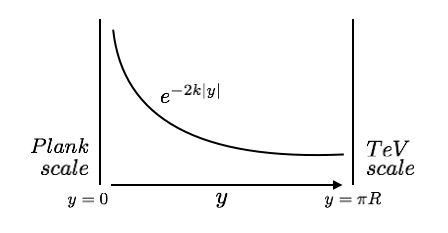
\includegraphics[width=0.6\textwidth]{branes}
    \caption{\label{brane}Diagram of the RS spacetime. ~\cite{R10}}
\end{figure}
%\shorthandon{=}  

In this thesis, $t^*$ is considered as a spin-3/2 Regge excitation desciribed by a Randall-Sundrum scenario given in  ~\cite{R7}. It is discribe by the Lagrangian \ref{rarita} \cite{R13}, where ${\cal D}_{\nu} = \partial_{\nu}-ig{\cal A}_{\nu}$. The Lagrangian tells the interaction between the particles considered in this thesis. It can be understood from the Lagrangian  there are  two quarks and a photon at the same space-time point.

\begin{eqnarray}
\label{rarita}
% \nonumber to remove numbering (before each equation)
	{\cal L}_{4} \ = i \overline {\Psi_\mu} \gamma^{\mu\nu\rho} {\cal D}_{\nu}{\Psi_\rho}+{\cal M}\overline {\Psi_\mu} \gamma^{\mu\rho} {\Psi_{\rho}}
%
%
\end{eqnarray}

For $t^*$$\rightarrow$$t$+$\gamma$ analysis, it is assumed that it has 100$\%$ branching fraction over other channels such as $t^* \rightarrow t+Z$ and $t^* \rightarrow t+g$ . Only pair production of $t^*$ is considered because it has a higher production cross section than single production of $t^*$ at the LHC. The reason for this is suppression of mixing between spin-3/2 and spin-1/2 states \cite{R7,R11}. It should be noted that despite considiration of a spin-3/2 RS resonance, the analysis is performed in a model independent way.

\chapter{Experimental Setup}
\section{LHC}
LHC \cite{R1} is the largest accelerating machine in the world. Also LHC is the worlds highest energy accelerator with its 27 km circle which is designed to accelerate protons up to a center of mass energy 14TeV. The source of protons in the LHC is a tube of hydrogen gas. After protons are separated from hydrogen gas, they are send to a Duoplasmatron to reach 90 KeV. Then they start their journey with entering radio frequency quadrupole (RFQ) and continue with LINAC2 here they reach up to 50 MeV. After then they enter PS (1.4 GeV $\rightarrow$ 26 GeV ) then in to SPS (26 GeV $\rightarrow$ 450 GeV). After this step they reach sufficient energy to enter LHC. With LHC, protons reach 8 TeV CM energy to simulate the similar state after the big bang. One can see schema of this journey in Figure \ref{LHC} . Two high-energy particle beams traveling at the speed 0.99999991c are focussed, bent and accelerated simultaneously during their journey.

\begin{figure}  [!htbptbp]
\centering
    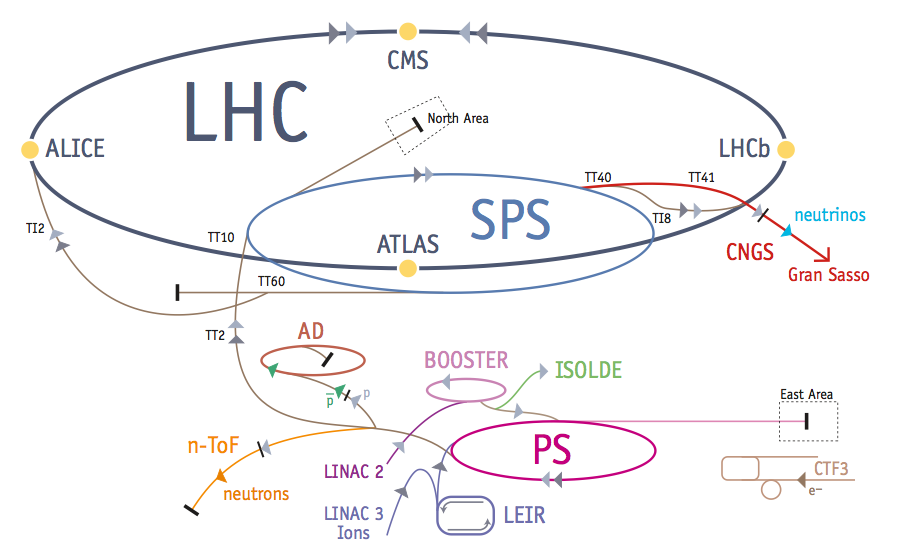
\includegraphics[width=0.8\textwidth]{LHC}
    \caption{\label{LHC}LHC complex. ~\cite{R1}}
\end{figure}

The particle beams collide at 4 interaction points in the LHC. These points contain also the 4 main detectors of LHC : A Large Ion Collider Experiment (ALICE), A Toroidal LHC Apparatus (ATLAS), Compact Muon Solenoid (CMS) and the Large Hadron Collider Beauty Experiment (LHCb). 


\section{CMS}
CMS \cite{R2,R3} is one of the two general purpose detectors of LHC. One can say briefly that physics at the TeV scale, Higgs boson, BSM physics can be studied with CMS. 

CMS is a onion shape detector. Main components of the detector can be seen in the Figure \ref{CMS}. A super conducting magnet (4T) is covering inner tracker and 2 calorimeters because large bending power is necessary in order to measure precisely the momentum of high-energy charged particles.

\begin{figure}  [!hbt]
\centering
    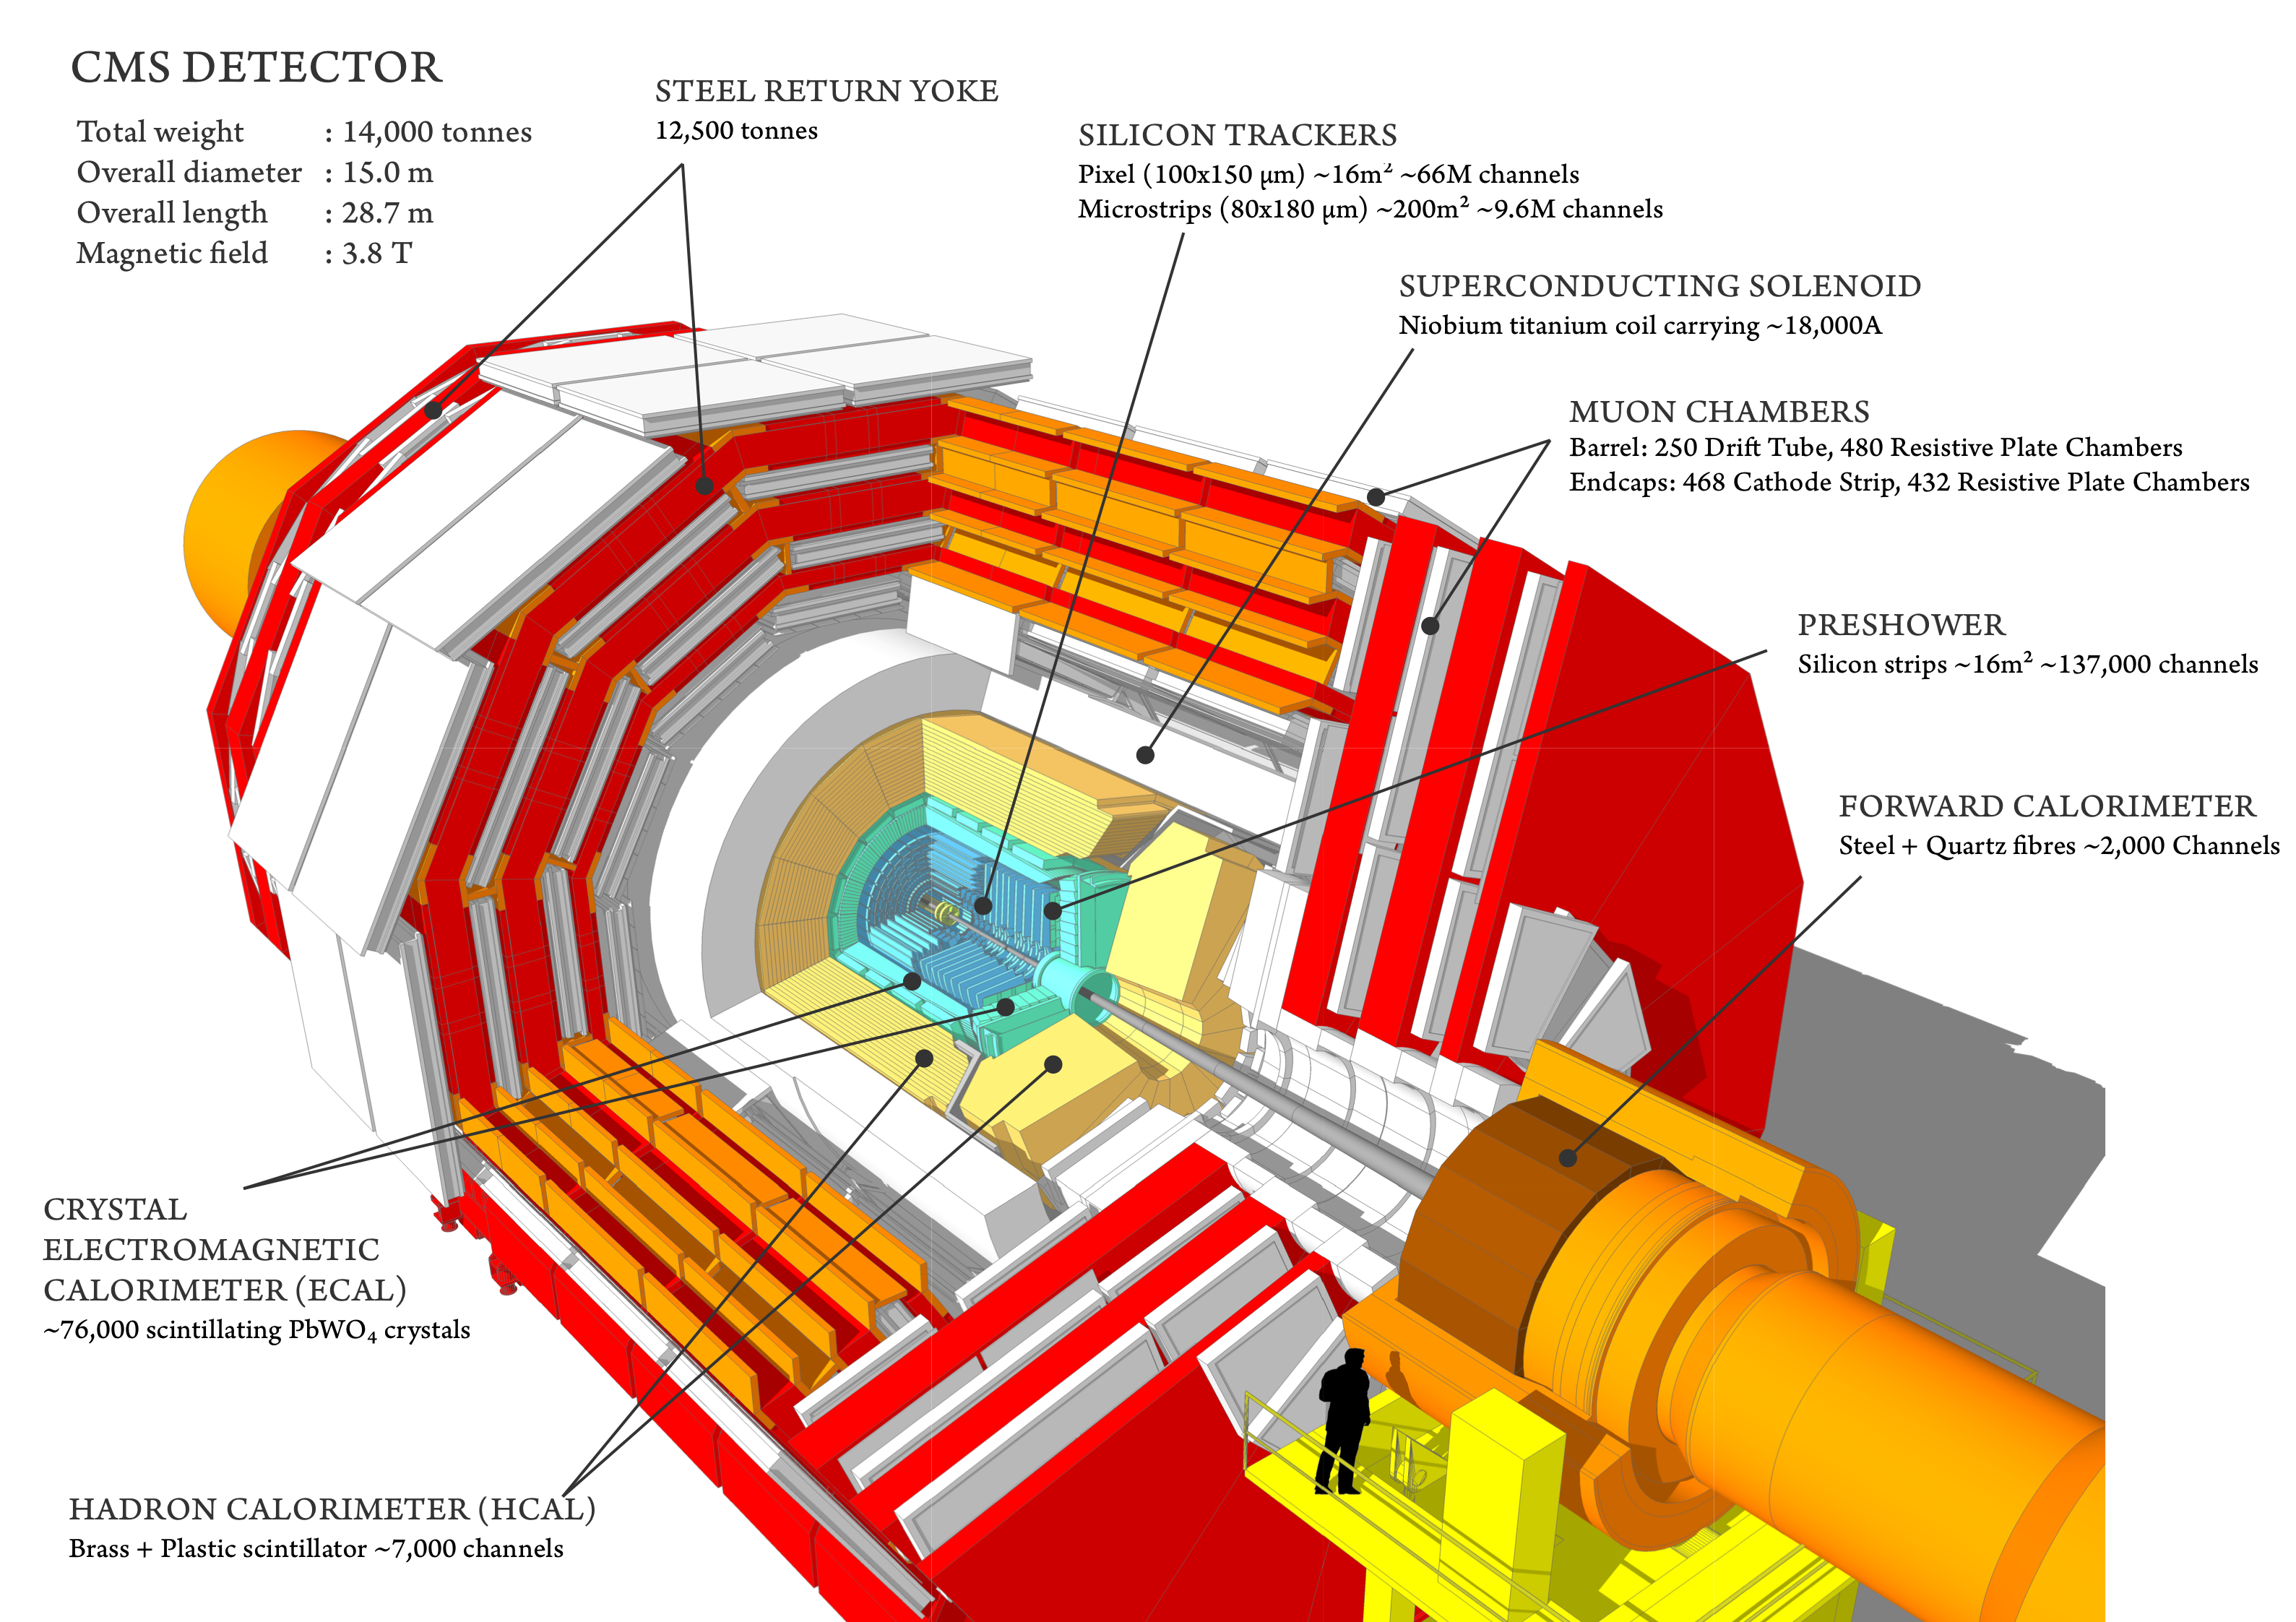
\includegraphics[width=0.8\textwidth]{CMS}
    \caption{\label{CMS}CMS Detector sectional view. ~\cite{R2}}
\end{figure}

In this point it is useful to explain CMS general geometry in other words coordinate system. The proton beam line is along the Z-axis which points tangentially with respect to center of LHC circle. Y-axis is vertical and points up. Because of the ring shape of LHC and cylindrical structure of CMS it is essential to use a different kinematic variable called pseudo-rapidity which is defined by polar angle $\eta$ in Formula \ref{eta}.

\begin{eqnarray}
\label{eta}
% \nonumber to remove numbering (before each equation)
	\eta=-\ell n [\tan(\frac{\theta}{2})]
\end{eqnarray}

It is important to introduce $\eta$ to explain barrel, endcap and forward regions of the detector. In addition to $\eta$ there is one more variable $\Delta R$ to determine angular distance. $\Delta R$ can be defined as a combination of distance between azimuthal angle($\phi$) and ($\eta$) as in the Formula \ref{deltar}.

\begin{eqnarray}
\label{deltar}
% \nonumber to remove numbering (before each equation)
	\Delta R = \sqrt{(\Delta\eta)^2 + (\Delta\phi)^2}
\end{eqnarray}

\begin{figure}  [!hbt]
\centering
    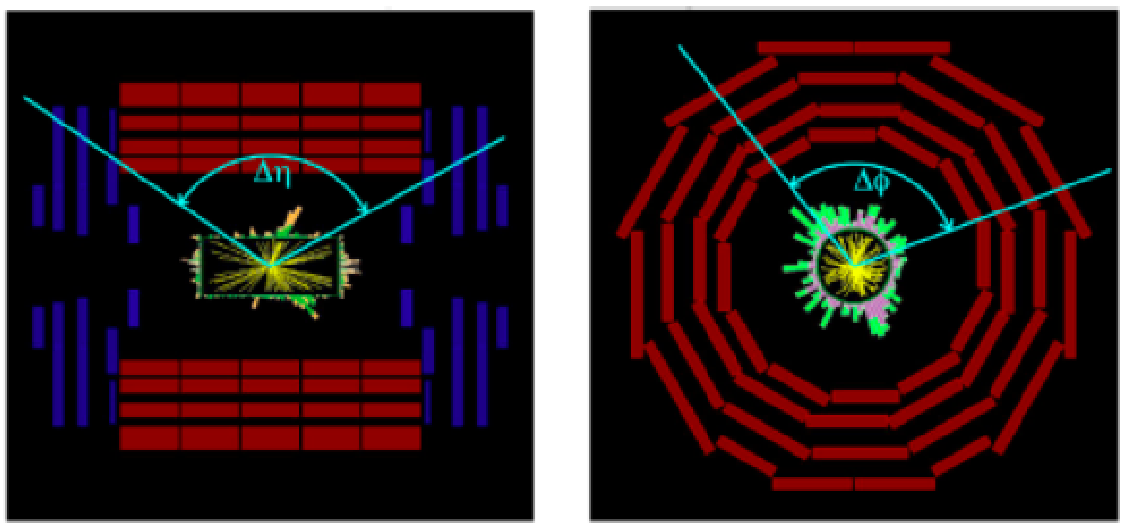
\includegraphics[width=0.8\textwidth]{DeltaR}
    \caption{\label{DeltaR} Definition of azimuthal angle($\phi$) and ($\eta$).}
\end{figure}

Additionally, as a note, it can be said that since there is no instrument along the beamline which is on the z direction, z component of particle momenta can only be measured indirectly.

\subsection{Inner Tracking System}

The innermost detector component is Tracker made entirely of silicon. In Figure \ref{Tracker} , there are 3 layers of pixel detector (in purple), 10 layers of silicon microstrip detectors (in red and blue) in the central region and 2 layers of pixel, 12 layers of silicon microstrip detectors in the endcaps to provide a good resolution.  Transverse impact parameter resolution of charged particles reaches 10$\mu$m for high $P_{T}$ tracks. Thus, CMS tracker is very good at determining the position of secondary vertices which is important to tag $b$ jets. 

For this analysis tracker has an important role in determining leptons $P_{T}$ and it is also important to measure jet energies by matching associated tracks.

\begin{figure}  [!hbt]
\centering
    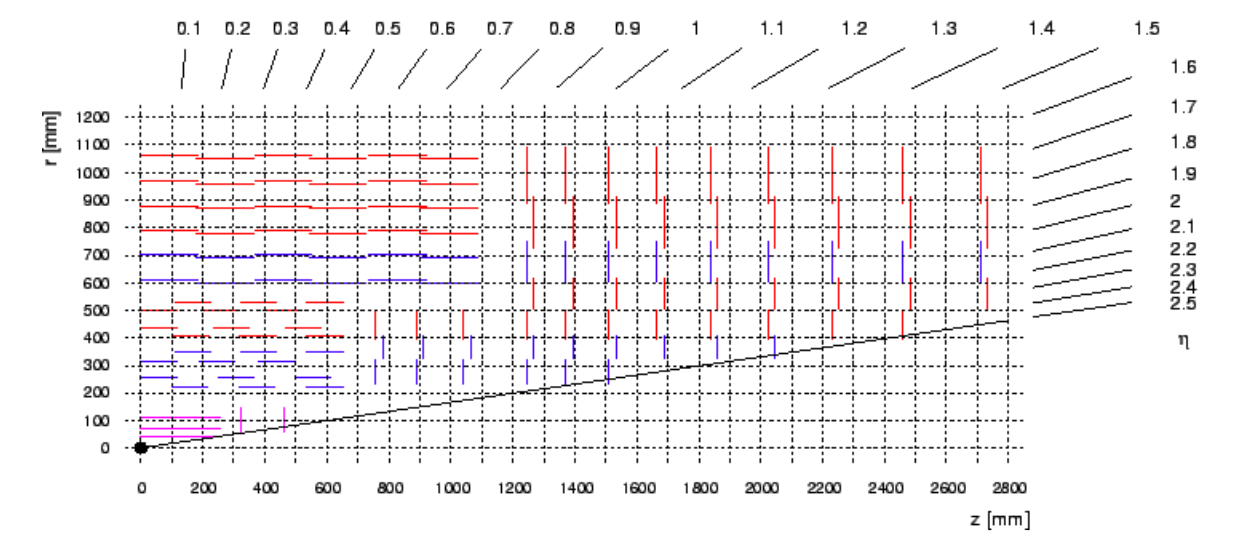
\includegraphics[width=0.8\textwidth]{Tracker}
    \caption{\label{Tracker}One quarter of the CMS Tracker layout. ~\cite{R15}}
\end{figure}

\subsection{Electromagnetic Calorimeter}

The electromagnetic calorimeter (ECAL) has pseudo-rapidity |$\eta$| < 3 and measures energy of the particles interacting electromagnetically like electrons and photons which play an important role in this analysis. In order to measure energy precisely ECAL is composed of 61200 lead tungstate (PbWO4) crystals. These crystals with their characteristics permit a fine granularity and compactness \cite{R16}. The region with |$\eta$| < 1.48 is reserved for the ECAL barrel (EB) and The ECAL endcaps (EE) positioned in the region 1.48 <|$\eta$|< 3.0 . 

\begin{figure}  [!hbt]
\centering
    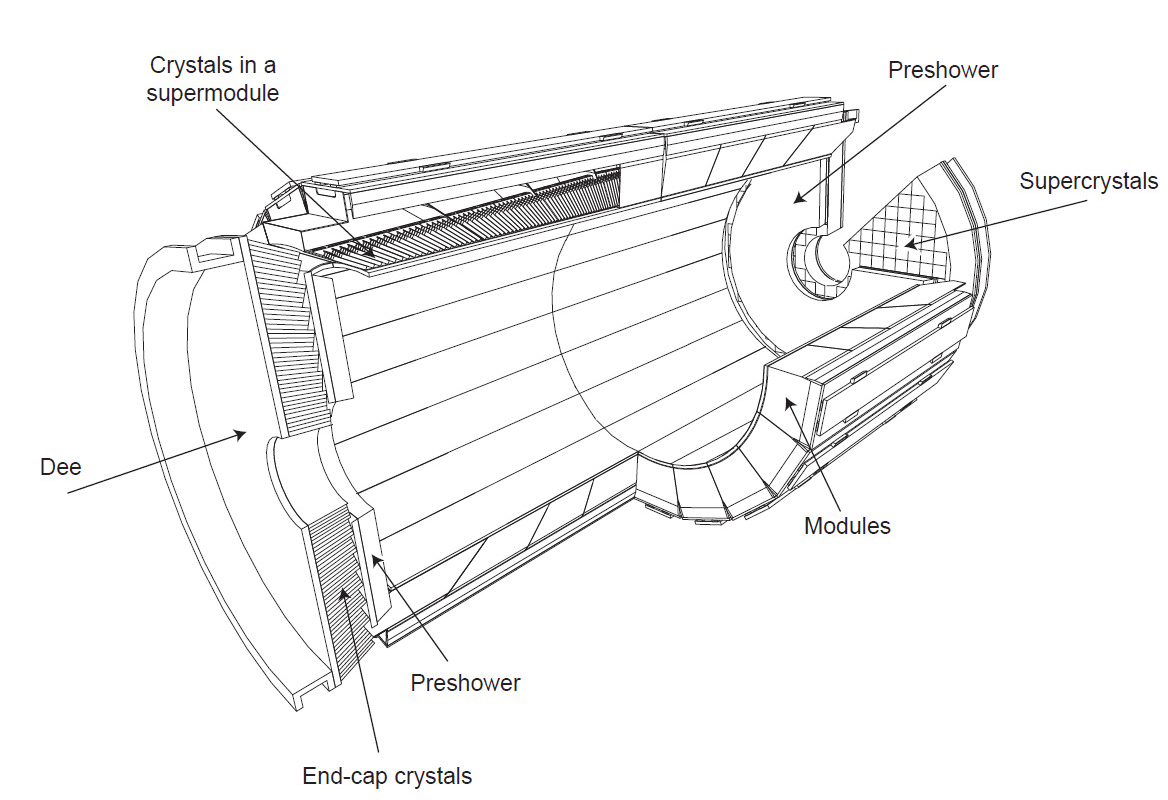
\includegraphics[width=0.8\textwidth]{ECAL}
    \caption{\label{ECAL}Layout of the CMS electromagnetic calorimeter presenting the arrangement of crystal modules, supermodules, endcaps and the preshower in front ~\cite{R16}.}
\end{figure}

The energy resolution of both EB and EE, can be recontructed by the Formula \ref{ecalenerji} where E is in GeV \cite{R16}. 

\begin{eqnarray}
\label{ecalenerji}
% \nonumber to remove numbering (before each equation)
	(\frac{\sigma}{E})^2 = (\frac{S}{\sqrt{E}})^2 + (\frac{N}{E})^2 + C^2
\end{eqnarray}

(S) is called the stochastic term presenting the event-to-event fluctuations, photoelectron statistics, and other fluctuations in the energy deposited in the preshower absorber. (N) is the noise term corresponding to electronic, digitization, dark current and pileup noise.  The light collection non-uniformity, errors on the inter-calibration among the modules, and the energy leakage from the back of the crystal are shown with the constant term (C). For example in 2004 barrel super model was tested with an electron beam having momenta between 20 and 250GeV/c. As a result of this test S,N,C were calculated as 2.8$\%$, 0.12, 0.30$\%$ respectively.


\subsection{Hadron Calorimeter}

ECAL is surrounded by hadronic calorimeter (HCAL) which is a brass/scintillator sampling hadron calorimeter within the same pseudo-rapidity as ECAL. HCAL exists due to measure energy of the particles made of quarks and gluons. In other words, HCAL measures energy of hadroniclly interacting particles.

Figure \ref{HCAL} shows the longitudinal view of the CMS HCAL dedector where one can easily see the locations of hadron barrel (HB), hadron outer (HO), hadron endcap (HE) and hadron forward (HF) components of the dedector. 

\begin{figure}  [!hbt]
\centering
    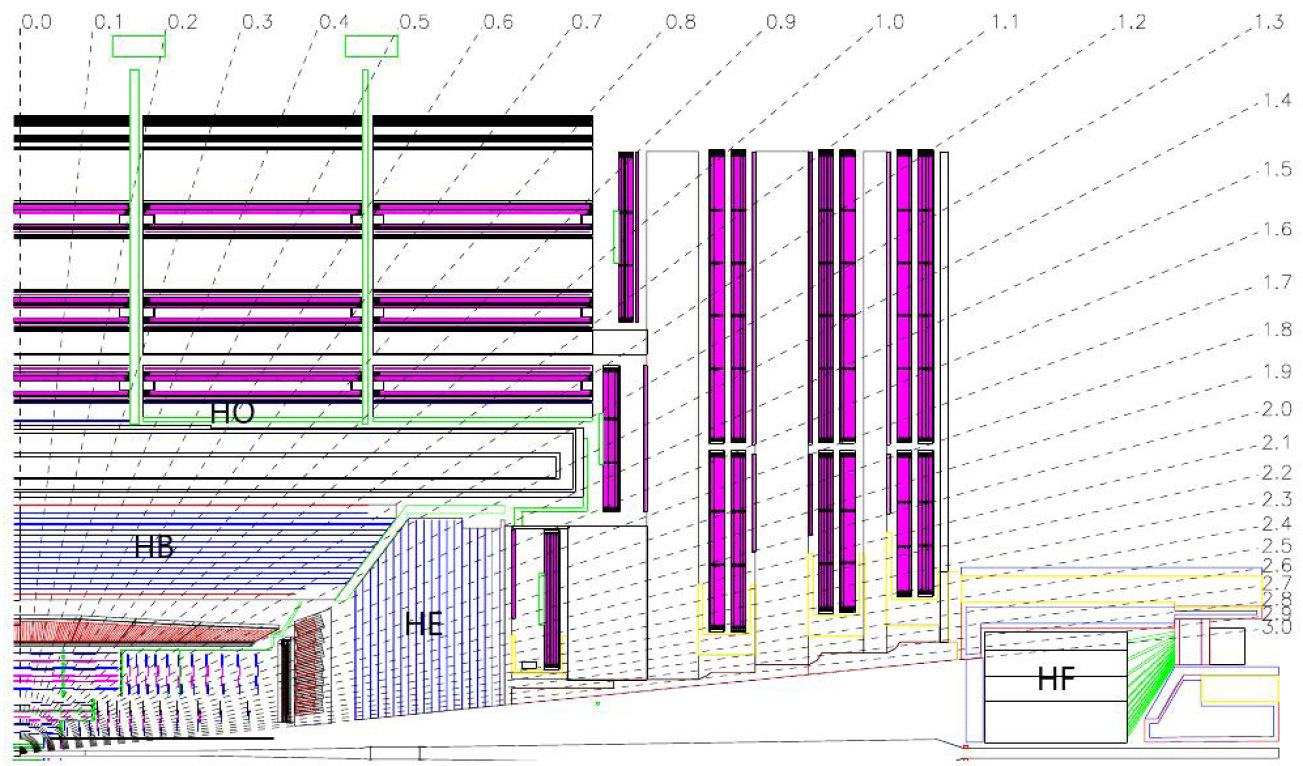
\includegraphics[width=0.8\textwidth]{HCAL}
    \caption{\label{HCAL}One quarter of HCAL Longitudinal view. The dashed lines are fixed $\eta$ values ~\cite{R16}.}
\end{figure}

Due to the fact that initial transverse momentum of protons is zero, it should remain zero after the collision. By considering this fact Missing Transverse Energy (MET) can be measured with the help of HCAL and ECAL \cite{R17}. Determining MET is very crucial for new physics searhes and also for this search to measure the $W$ boson mass via leptonic channel.

Measurement of direction and energy of particle jets can be also done by considering ECAL and HCAL results simultaneously \cite{R17}.  
The energy resolution obtained from test on combination of ECAL and HCAL is given by the Formula \ref{EHenergy} which gives approximately 5mm width of EM shower when pion is used with enegy interval from 150 to 300 GeV \cite{R16}.

\begin{eqnarray}
\label{EHenergy}
% \nonumber to remove numbering (before each equation)
	(\frac{\sigma}{E})^2 = (\frac{70\%}{\sqrt{E}})^2 + (8\%)^2
\end{eqnarray}

\subsection{The Muon System}

The outermost layer is muon chamber composed of four muon station spaced with iron “return yoke” plates. The muon chamber also is a tracking device and because it is in the outermost region of CMS no other particles except muons and neutrinos can reach this section. Thus, reconstruction of  the muons are fast and highly efficient \cite{R16}. In addition to this muon charge can be determined with the help of bending direction in the magnetic field, positively and negatively charged particles are bending in opposite directions. 

\begin{figure}  [!hbt]
\centering
    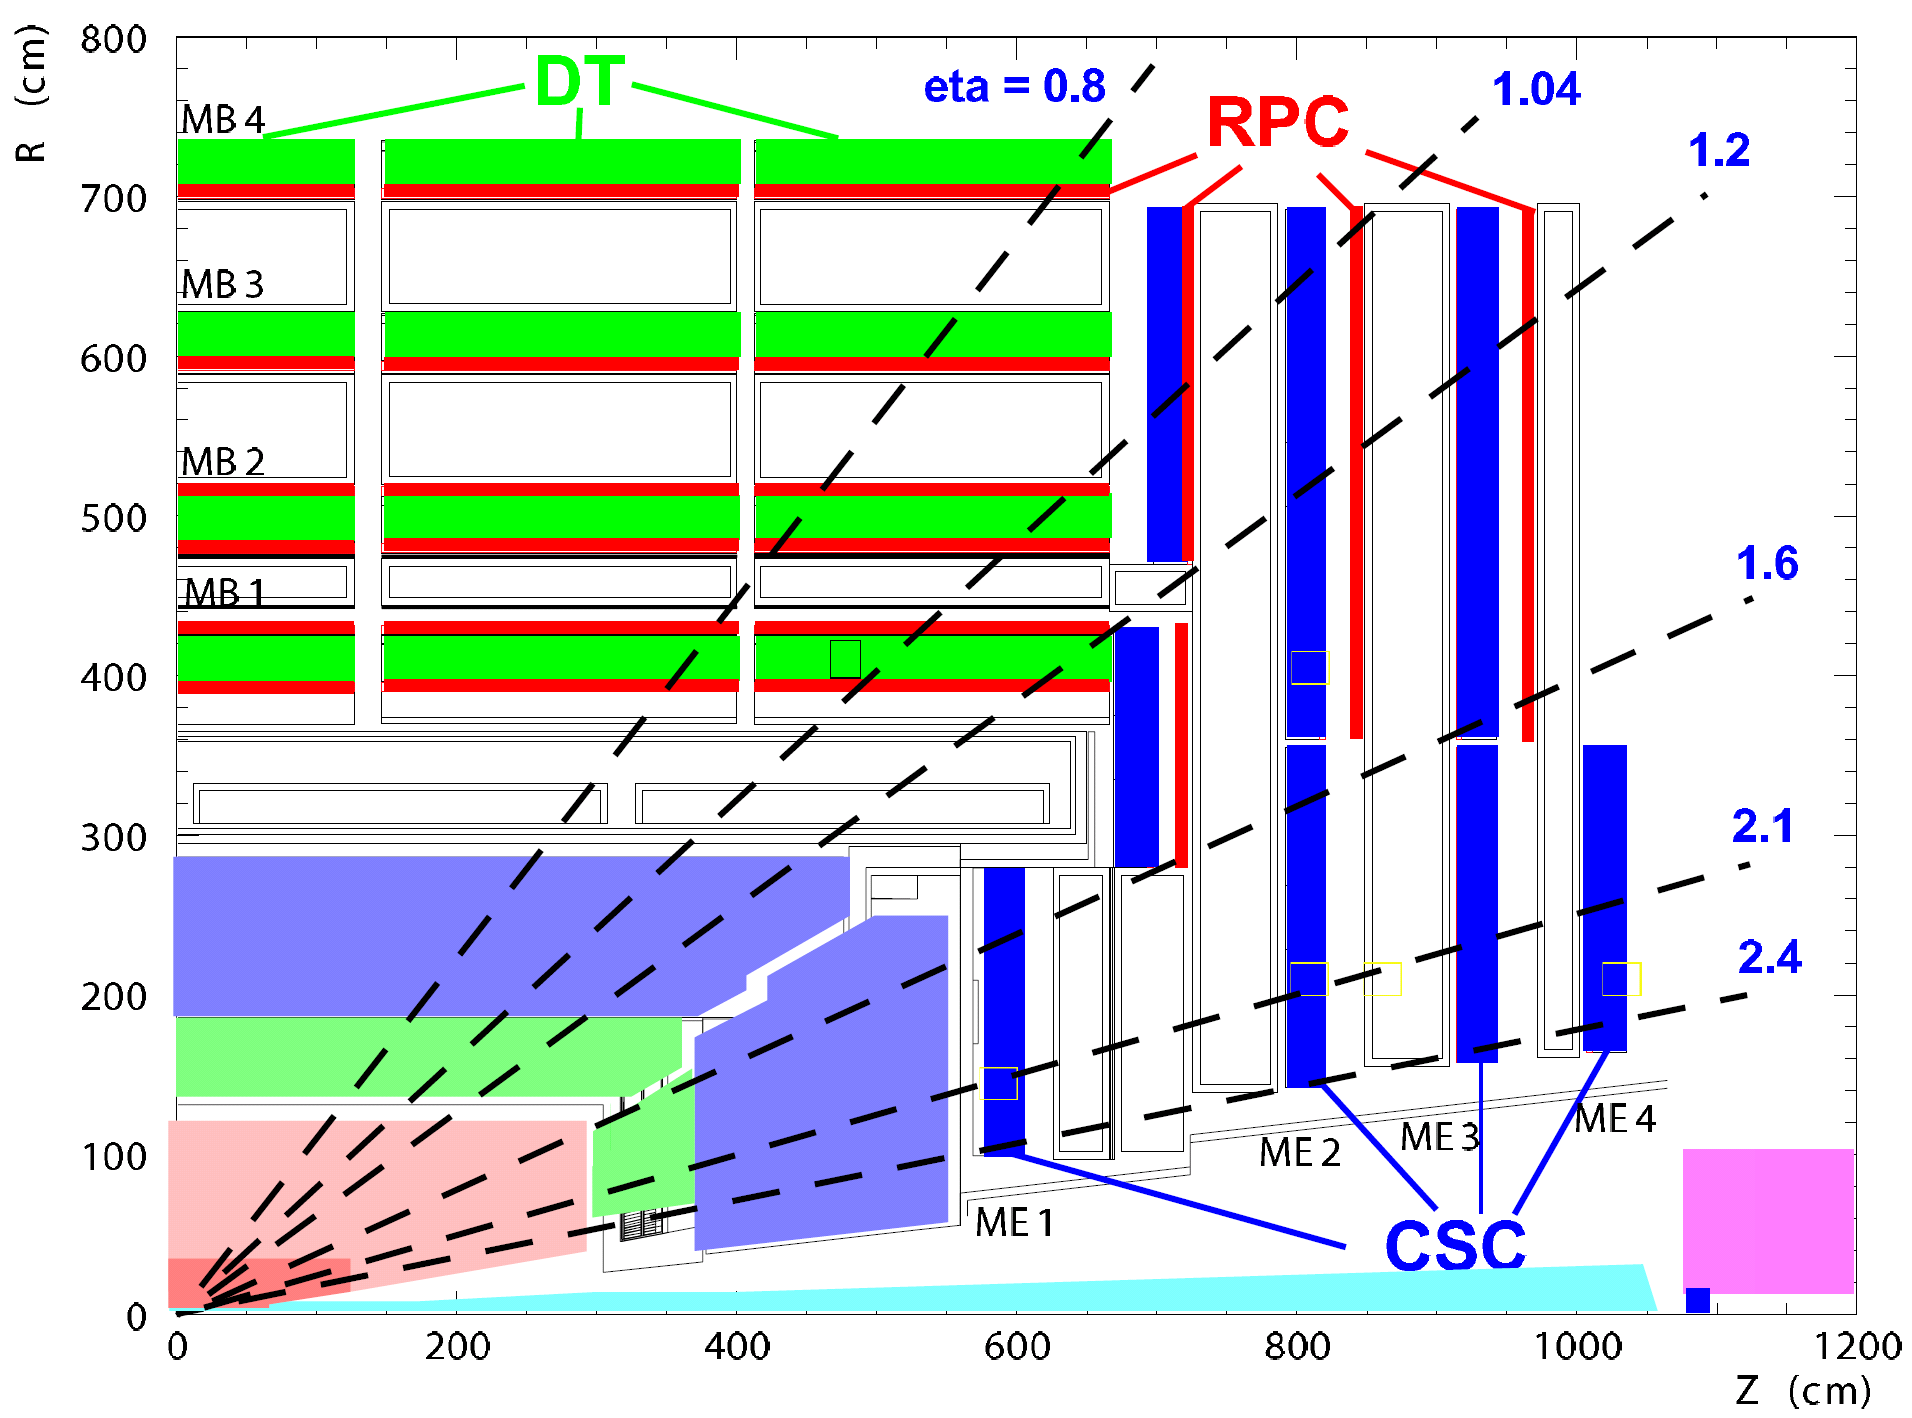
\includegraphics[width=0.8\textwidth]{muon2}
    \caption{\label{muon2}A longitudinal view of the muon system indicating the location of the three detector types of the muon system. Dashed lines represent fixed $\eta$ ~\cite{R16}.}
\end{figure}

Figure \ref{muon2} shows the muon system of the CMS dedector is a combination of three dedector: Drift Tubes (DT), Cathode Strip Chambers (CSC) and Resistive Plate Chambers (RPC). 

\subsection{Trigger and Data Acquisition System}
\label{triggerexp}
There are many challenges for Trigger and Data Acquisition (TDAQ) system at LHC. Some of these are enormous data rate (40 MHz of collisions), production of approximately 20 event per bunch crossing which means 1Tbyte of zero suppressed data in CMS readout system and the crossection is very small for new physics.  In order to collect data at this high rate, CMS has a complex TDAQ system as seen in the Figure \ref{tdaq} at left. On the other hand it can be explained in a simplier way as in the Figure \ref{tdaq} at right. CMS has only two  trigger levels, L1 trigger and High Level Trigger (HLT). Event rate of 40 MHz is reduced to 100kHz by L1 trigger system to be passed to HLT system. There are intermediate event building step (readout buffers) and large network switching between L1 and HLT. HLT is a software system that makes event rate decreases 100Hz and this results in a data rate of 150 Mbyte per second.


\begin{figure}  [!hbt]
\centering
    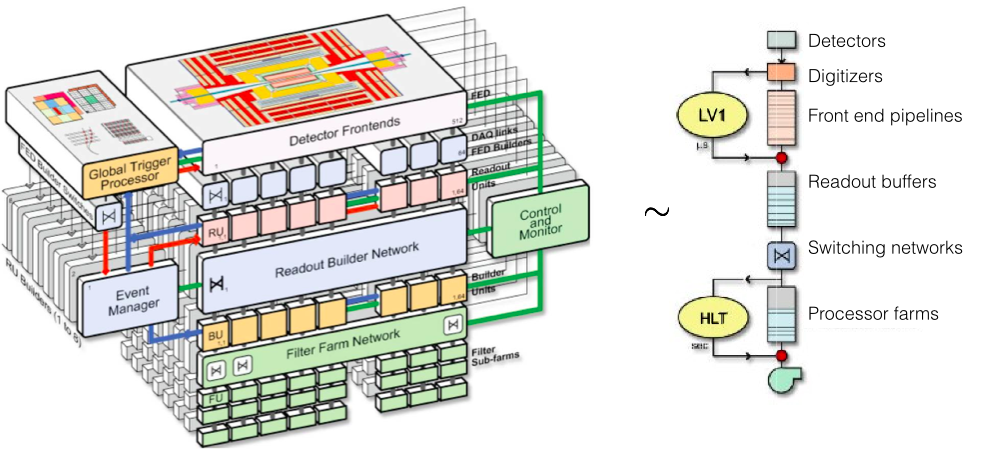
\includegraphics[width=0.8\textwidth]{tdaq}
    \caption{\label{tdaq}General tdaq structure of CMS (left), summarised tdaq structure of CMS(right) ~\cite{R16}.}
\end{figure}

\subsection{Computing}
The most important part of CMS computing system is CMS software (CMSSW) stands for online data taking, simulation, primary reconstruction, and physics analysis \cite{R16}. Since CMSSW composed of many subpackages related to physics analysis, complicated analysis steps become much simpler. There are also a lot of beneficial functions specific to CMS, for example CMSShape is used in this analysis to fit Background data (detailed in sec. \ref{fakerateleptons} ). 

Some crucial steps have to be performed in order to reach data analysis stage. After filtering the first data with the help of L1 trigger and HLT,  the process of selecting events and saving them in output is performed which is called skimming. This dedector output is RAW data from which the physics object reconstructed by a second skimming. Now this new data is called reconstructed (RECO) data. RECO data includes reconstructed objects such as tracks, vertices, jets, electrons, muons, hits/clusters. Moreover, there is Analysis Object Data (AOD) derived from RECO data, to provide data for physics analysis in a convenient, compact format \cite{R18}. Physics analyses can directly use AOD Data. All these RAW, RECO and AOD tiers can be seen in figure ~\ref{data1}.
It should be noted that data formants of CMS are in ROOT format which is a C++ based framework for data processing.

\begin{figure}  [!hbt]
\centering
    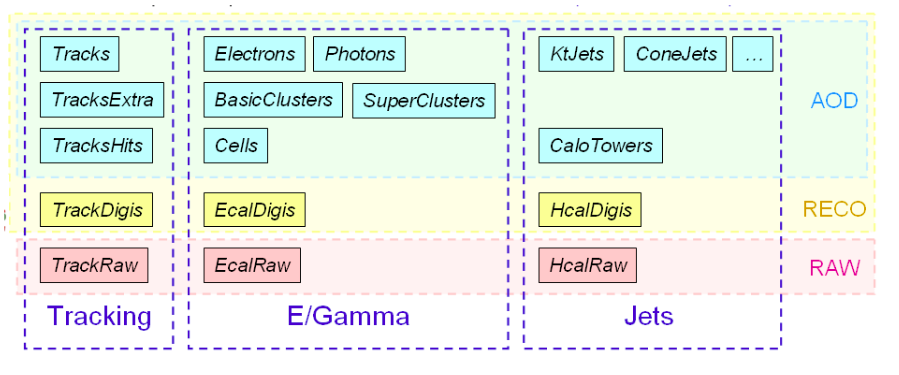
\includegraphics[width=0.8\textwidth]{data}
    \caption{\label{data1}DATA tiers of CMS ~\cite{R18}.}
\end{figure}

%%%%%%%%%%%%%%%%%%%%%%%%%%%%%%%%%%%%%%%%%%%%%%%%%%%%%%%%%%%%
%%%%%%%%%%%%%%%%%%%%%%%%%%%%%%%%%%%%%%%%%%%%%%%%%%%%%%%%%%%%
%%%%%%%%%%%%%%%%%%%%%%%%%%%%%%%%%%%%%%%%%%%%%%%%%%%%%%%%%%%%
\chapter{Analysis}

In this thesis, a search for a pair produced excited quark ($t^*$ ) is performed using proton-proton collision data collected by CMS at 8 TeV corresponding to an integrated luminosity of 19.6${fb}^{-1}$. In this analysis, $t^*$ decays exclusively to a top quark and a photon. Figure \ref{signal} shows that analysis is performed in semi-leptonic channel. In the final state  there are two isolated photons, at least 4 well-reconstructed jets and one lepton, which can be either a single isolated muon or electron. Analysis is performed in a model independent way while a heavy spin-3/2 excitation of a heavy spin-1/2 quark indicated by ”Rarita-Schwinger” vector spinor Lagrangian is the most favourable choice among other beyond the standard models.

In this chapter, before focussing on how the analysis is performed, Monte Carlo (MC) and data samples used in this search and corresponding computing tools will be presented. Then, ${\chi}^2$ sorting and Matrix method with tag and probe technique will be explained in a detailed fashion.

\begin{figure}[!hbt]
\centering
    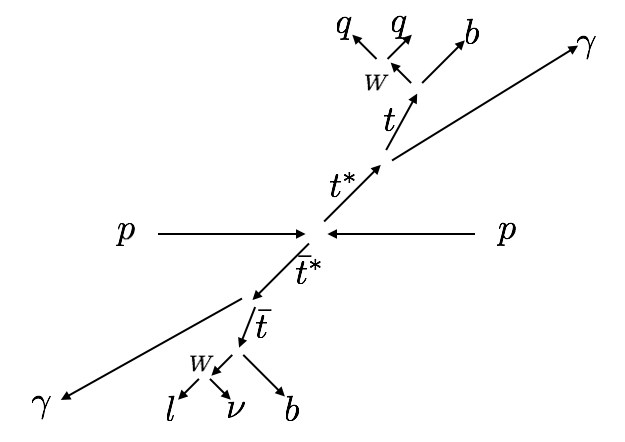
\includegraphics[width=0.8\textwidth]{signal}
    \caption{\label{signal} t* decays to top quark and a photon semi-leptonicly.}
\end{figure}

\section{MC and Data Samples}

The proton-proton collision events with a CM energy of 8 TeV are used for this analysis, measured with the pixel subdetector information. These events were collected using muon or electron triggers (detailed in), and reconstructed using CMS software \footnote{Version CMSSW$\_$5$\_$3$\_$7$\_$patch5}. Data Sets processed for this analysis are shown in Table \ref{DATASets}.

Signal efficiencies are predicted using simulated samples.The pair production of $pp \rightarrow t^* \overline{t}$* signal process is simulated, including up two additional hard partons, using the MADGRAPH \cite{Mad} event generator and the CTEQ6L1 \cite{Cteq} parton distribution functions (PDFs) and then passed to PYTHIA \cite{Pythia} for hadronization. Moreover, dedector simulation is performed using GEANT4 \cite{Geant} in CMSSW \footnote{Version CMSSW$\_$5$\_$3$\_$2$\_$patch4}.

\begin{table}[!hbt]
\caption{Summary of 8 TeV collision data streams used in this analysis, along with their run ranges and integrated luminosity}
\label{DATASets}
\begin{center}
\begin{tabular}{l | c c} %\hline
		 Dataset & Run Range & ${\cal L}(pb^{-1})$ \\ \hline
\\
 /MuHad/Run2012A-22Jan2013-v1  & 190645–193621 & 876.2\\ %\hline
/SingleMu/Run2012B-22Jan2013-v1 & 193834–196531 & 4411.7 \\
/SingleMu/Run2012C-22Jan2013-v1 & 198049–203002 & 7055.2 \\
/SingleMu/Run2012D-22Jan2013-v1 & 203709–208686 &  7369.0 \\
/ElectronHad/Run2012A-22Jan2013-v1  & 190645–193621 & 876.2 \\
/SingleElectron/Run2012B-22Jan2013-v1  & 193834–196531 &  4411.7 \\
/SingleElectron/Run2012C-22Jan2013-v1 & 198049–203002 & 7055.2 \\
/SingleElectron/Run2012D-22Jan2013-v1 & 203709–208686 & 7369.0
\\ %\hline
\end{tabular}
\end{center}
\end{table}


\section{Signal Reconstruction}

Event reconstruction is performed by using Particle Flow (PF) \cite{PF1,PF4} algorithm which combines the information of all CMS subdetectors to reconstruct and identify all stable particles in an event such as electrons, muons, photons, charged hadrons and neutral hadrons. The PF algorithm first reconstructs the central elements which are the charged particle tracks, calorimeter clusters, and muon tracks. Then they are linked into blocks and interpreted as particles. Since a particle can be detected in various subdetectors, the PF elements must be connected with each other, which is done with a linking algorithm to avoid double counting. The last step consists of reconstructing and identifying particles based on the blocks of elements.

\subsection{Reconstruction of elements}
\label{elements}

\begin{itemize}

\item Trigger \cite{trigger}: The events passing through triggers (L1 and HLT) explained in section \ref{triggerexp}, which look for a high $P_T$ lepton and at least three jets in an event, were analyzed. 

\item Primary vertex reconstruction: The presence of a primary vertex, which is consistent with the beamspot position, can indicate a collision happening. The noncollision backgrounds, such as beam halo and cosmic-ray muons, can be vetoed by requiring a primary vertex. The primary vertex can be well-reconstructed by following:
more than 10 tracks originating from it, with at least 25$\%$ of those being high purity; at least 4 degrees of freedom; an impact parameter with respect to the beamspot in $z$, $d_z$, that satisfies |$d_z$|<24 cm; an impact parameter with respect to the beamspot in the $xy$ plane, $d_{xy}$, that satisfies $d_{xy}$<2cm.

\item Lepton Reconstruction: \\
\underline{Muon reconstruction and selection:} 
Muons are initially reconstructed by identifiying hits in the different layers of the muon chamber such as drift tubes and the CSCs. There are two different approaches, global muons and tracker muons, to construct straight line track segments in the local reconstruction by using hits. These tracks can be either based on hits in the muon dedector alone or a combination of hits in the muon dedector with in the central dedector. The latter muons are called global muons. When low $P_T$ (<5GeV) muons are considered, using tracker muons are more efficient. On the other hand, since the algorithm makes use of full bending power of the CMS magnetic field, resolution of high $P_T$ global muons is better. Thus, in this search muons are reconstructed as a global muon. Addtionally, muon are selected with $P_T$ >20GeV/c, |$\eta$|<2.1, tight tag of the muon physics object group (POG) \cite{R21}. Multiplicity distribution for muon is given in Figure \ref{Nmuons}

\begin{figure}[!hbt]
\centering
    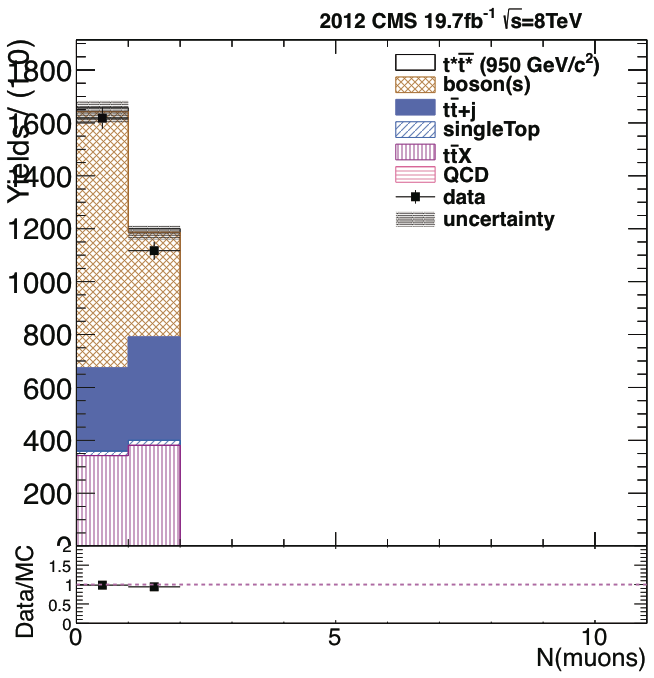
\includegraphics[width=0.8\textwidth]{Nmuons}
    \caption{\label{Nmuons} Multiplicity distribution for muon.}
\end{figure}

\underline{Electron reconstruction and selection \cite{electron}:}
In CMS electrons leave their signatures both in the tracker and ECAL. This signature is an energy deposite in ECAL which collects bremsstrahlung photons emitted along
the electron trajectory in the tracker volume. A cluster driven pixel hit matching algorithm with with a Gaussian Sum Filter is used to determine energy and momentum of electron in CMS. The electron energy is deduced from a weighted combination of the corrected supercluster energy and tracker momentum measurements. The electron direction is that of the reconstructed electron track at interaction vertex. In this search, ellectrons tagged as tight by egamma POG are selected. Moreover,  $P_T$ >30GeV/c, |$\eta$|<2.4 cuts are applied to recontructed electrons and since there is a transition region between barrel and endcap electrons in that region (1.4442<|$\eta$|<1.566) are not taken under consideration. Multiplicity distribution for electrons is given in Figure \ref{Nelectrons} 

\begin{figure}[!hbt]
\centering
    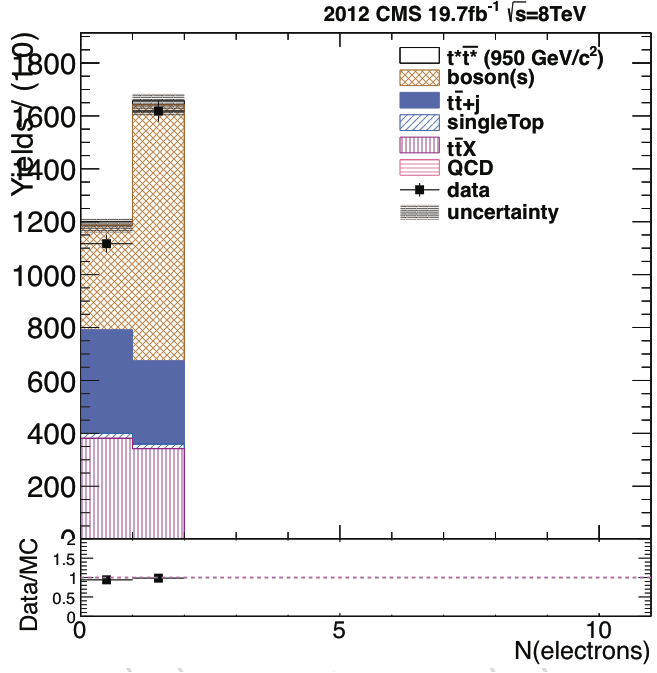
\includegraphics[width=0.8\textwidth]{Nelectrons}
    \caption{\label{Nelectrons} Multiplicity distribution for electron.}
\end{figure}

In addition to electron and muon selection, a simple cleaning cut is applied to distinguish electrons from muons ($\Delta R$(muons,electrons)>0.3).

\item Photon Reconstruction and Selections \cite{photon}: 
In this analysis, there are two isolated photons to be reconstructed. Photons can be reconstructed with a very good energy resolution in CMS by means of the ECAL granularity, tracker, and the large magnetic field. Charge particles are bending with the magnetic field and with granularity of ECAL photons can be seperated well from the charged particles. The photons identification made by egamma POG is mainly based on isolation, shower shape variables, and the ratio of energy deposits in the single hadronic calorimeter tower divided by the energy deposits in the single electromagnetic calorimeter tower ($H/E$). As in electron selection case, photons  tagged as tight by egamma POG are selected. Moreover,  $P_T$ >30GeV/c, |$\eta$|<2.5 cuts are applied and again photons in th region 1.4442<|$\eta$|<1.566 are vetoed. 

Additionally, a simple cleaning cut is applied to distinguish photons from leptons ($\Delta R$(photons,leptons)>0.3). Multiplicity distribution for photons is given in Figure \ref{Nphotons}.

\begin{figure}[!hbt]
\centering
    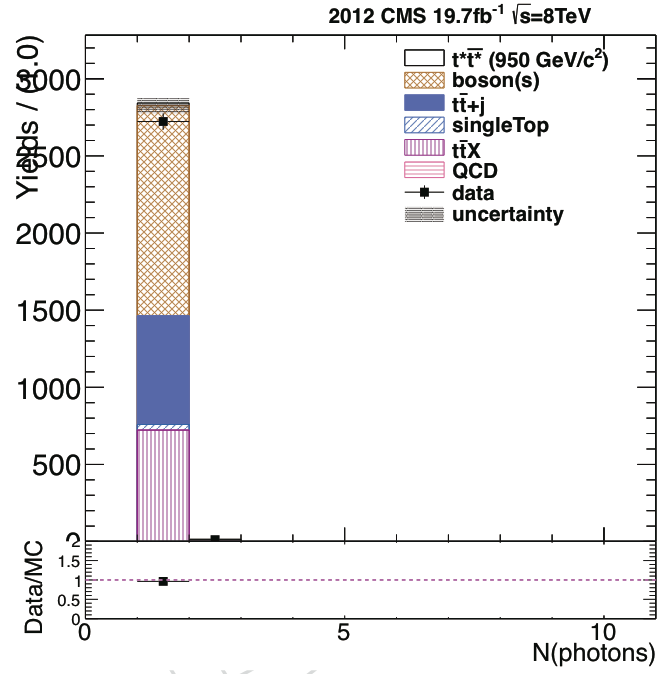
\includegraphics[width=0.8\textwidth]{Nphotons}
    \caption{\label{Nphotons} Multiplicity distribution for photon.}
\end{figure}

\item Jets Reconstruction and Selections \cite{jet}: 
There are a lot of definition for jets it can be simply said that jets are narrow hadron cones produced by quark or gluon hadronization and showering in dedector. Jet effect occurs due to quark confinement. An algorithm called anti-kt jet clustring algorithm \cite{antikt} is generally used for reconstructing original parton (gluon or quark) in CMS. This algorithm is used to measure distance ($d_{ij}$) between two particles with the Formula \ref{kt} where $k_{ti}$ is $i$th particle transverse momenta, $\Delta^2_{ij}$ = $(y_{i} - y_{j})^2$+$(\phi_{i} - \phi_{j})^2$, $\rho$ is a parameter to modify the relative power of the energy versus the geometrical ($\Delta_{ij}$) scales, and $R$ is the radius parameter. On the other hand, the distance between $i$th particle and beam is defined as $d_{iB}=k^{2\rho}_{ti}$. Among three different algorithm anti-kt is the one with $\rho$=1. Popularly in CMS, cone size is R=0.5.

\begin{eqnarray}
\label{kt}
% \nonumber to remove numbering (before each equation)
	d_{ij} = min(k^{2\rho}_{ti}, k^{2\rho}_{tj}) \frac{\Delta^2_{ij}}{R^2}
\end{eqnarray}

In this analysis, jets have $P_T$ at least 25 GeV/c and |$\eta$|<2.5. Jets, additionally, are required to pass PFjetID, this yields; neutral hadron fraction <0.99,  neutral electromagnetic fraction < 0.99, number of constituents >1. Moreover, as in the photon and lepton case, a simple cleaning cut is applied ($\Delta R$(jets,leptons)>0.5 and $\Delta R$(jets,photons)>0.5 ). Multiplicity distribution for jets is given in Figure \ref{NJets}

\begin{figure}[!hbt]
\centering
    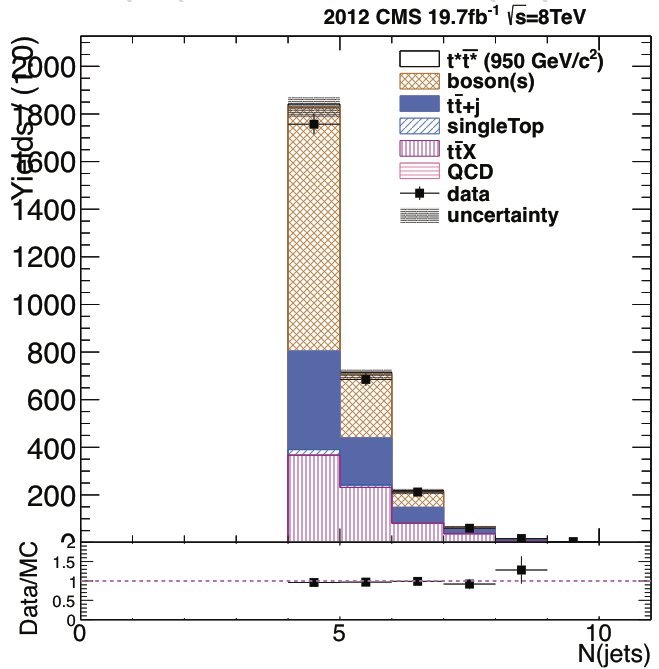
\includegraphics[width=0.8\textwidth]{NJets}
    \caption{\label{NJets} Multiplicity distribution for photon.}
\end{figure}

\item Pile-up reweighting and scale factors \cite{pileup}: 
Definition of Pile-up is dealing with multiple proton proton collisions in the same brunch crossing. There are three types of pile-up treatment depending on their time of entry in calorimeter system: in-time, out of time (late), out of time (early). In this analysis, in-time and out of time pile-ups for each bunch crossing are chosen from a Poisson distribution having a mean equal to the number of true interactions. MC samples are reweighted by using the true distributions from data and MC.

\item Event selection:
As in Figure \ref{signal},  $t^* \bar t$* $\rightarrow$ $WbW \bar b$ $\gamma \gamma$. A heavy quark ($t^*$) decays $t + \gamma$ with  a 100$\%$ percent branching ratio in semi-leptonic channel. On one side $W$ decays leptonically where the charged lepton can be either muon or electron, while on the other side $W$ decays 2 quarks. Therefore, selected events have exactly one electron or muon, one photons and at least 4 jets (2 from hadronic decay of W and 2 from b jets). All particles have to pass selection criterias explained before in this section.

\end{itemize}

\subsection{$\chi^2$ Sorting Method}
A $\chi^2$ sorting method is implemented  to reconstruct mass of $t^*$ within events passing selection criterias in previous section \ref{elements}. This method implies to choose events have minumum $\chi^2$ when all combimation of objects' reconstruntions are in consideration. Definition of  the $\chi^2$  is given in the Formula \ref{chi} where $W_{jj}$ consists of 2 jets while $W_{l\nu}$ includes a lepton and a neutrino, ${t_{w_{jj}+b}}({t_{w_{l\nu}+b}})$ is composed of $W_{jj}(W_{l\nu})$ plus a b jet, t* is the signal mass. 

\begin{eqnarray}
\label{chi}
% \nonumber to remove numbering (before each equation)
	{\chi}^2 = \frac{|M_{w_{jj}} - M_W|^2}{\sigma (W_{jj})^2} + \frac{|M_{t_{w_{jj}+b}} - M_{top}|^2}{\sigma ({t_{w_{jj}+b}})^2} 
+ \frac{|M_{t_{w_{l\nu}+b}} - M_{top}|^2}{\sigma ({t_{w_{l\nu}+b}})^2} \nonumber \\
+\frac{|t^*(t_{w_{l\nu}+b}+\gamma)-t^*(t_{w_{jj}+b}+\gamma)|^2}{\sigma(t^*_{lep})^2 + \sigma(t^*_{had})^2}
\end{eqnarray}

In the Formula \ref{chi}, $M$ refers to an objects mass and $\sigma$ indicates corresponding mass resolutions which are obtained by using MC truth information as in the Table \ref{massres}. Moreover, objects' masses are chosen as following according to PDG values: $M_W$ is 80.398 $GeV/ c^2$, and $M_{top}$ is 172.9 $GeV/ c^2$. Since $t^*$  mass is the one being searched, only mass difference of $t^*$s coming from two sides (leptonic and hadronic) is considered when calculating ${\chi}^2$ . 

\begin{table}[!hbt]
\caption{Mass resolutions which are obtained by using MC truth information}
\label{massres}
\begin{center}
\begin{tabular}{l | l} %\hline
		 & Mass Resolutions \\ \hline
\\
 $\sigma(W_{jj})$    & 9.296 $GeV/c^2$  \\ %\hline
$\sigma ({t_{w_{jj}+b}})$ & 16.49 $GeV/c^2$ \\
$\sigma ({t_{w_{l\nu}+b}})$ & 22.43 $GeV/c^2$ \\
$\sigma(t^*_{lep}) $ & 31.63 $GeV/c^2$ \\
$\sigma(t^*_{had}) $ & 31.59 $GeV/c^2$ \\
 %\hline
\end{tabular}
\end{center}
\end{table}

Since the transverse momenta of neutrino can be obtained from the missing transverse momenta in the experiment and since there is no machine on beam axis(z-axis), the longitudinal component of neutrino momentum needs to be calculated using a $W$ boson mass constraint. In this analysis, solution with the minumum ${\chi}^2$ is considered among two neutrino $p_Z$ solutions coming from $W$ boson mass constraint calculation (equation \ref{nupz}). In equation \ref{nupz} $W$ boson mass is already known and lepton for momentum can be calculated easily from dedector information. 

\begin{eqnarray}
\label{nupz}
% \nonumber to remove numbering (before each equation)
	P^2_W  = M^2_W = (P_{\nu} + P_{l})^2 = P^2_{\nu} + P^2_{l} + 2P_{\nu}P_{l}
\end{eqnarray}

MC study of this signal reconstruction is performed by scanning the invariant mass interval between  650 $GeV/c^2$ and 1000 $GeV/c^2$ one by one for each 50 $GeV/c^2$ mass step. Results for assuming that there is a signal at 800 $GeV/c^2$ are shown in figures \ref{Wlep}, \ref{Whad}, \ref{toplep}, \ref{tophad}, \ref{tstarlep}, \ref{tstarhad} respectively for each element of the $t^* \rightarrow t + \gamma$.

\begin{figure}[!h]
\centering
    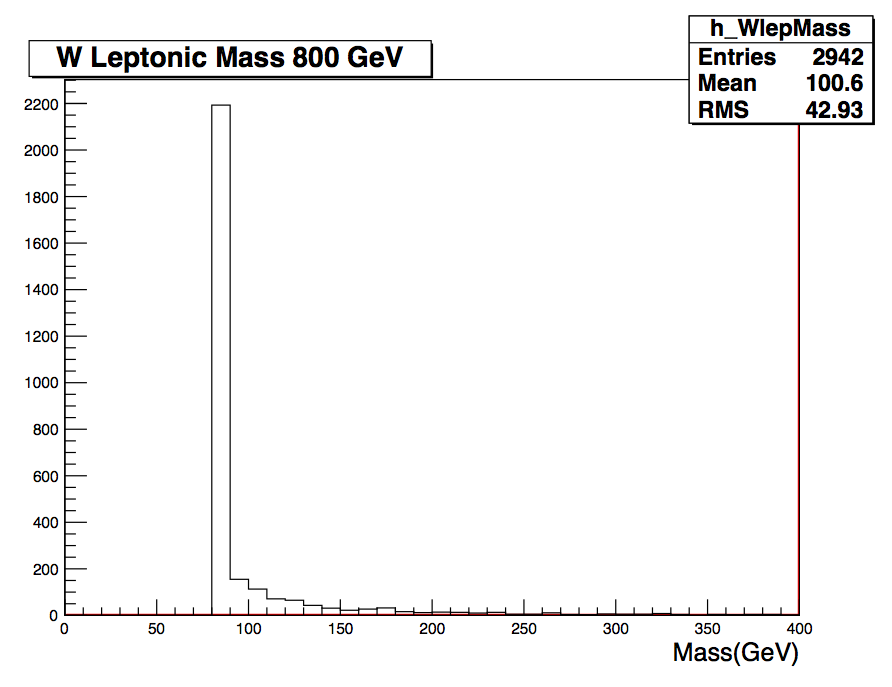
\includegraphics[width=0.8\textwidth]{Wlep}
    \caption{\label{Wlep} Invariant mass distribution of leptonic $W$ boson assuming there is a signal at 800 $GeV/c^2$.}
\end{figure}

\begin{figure}[!h]
\centering
    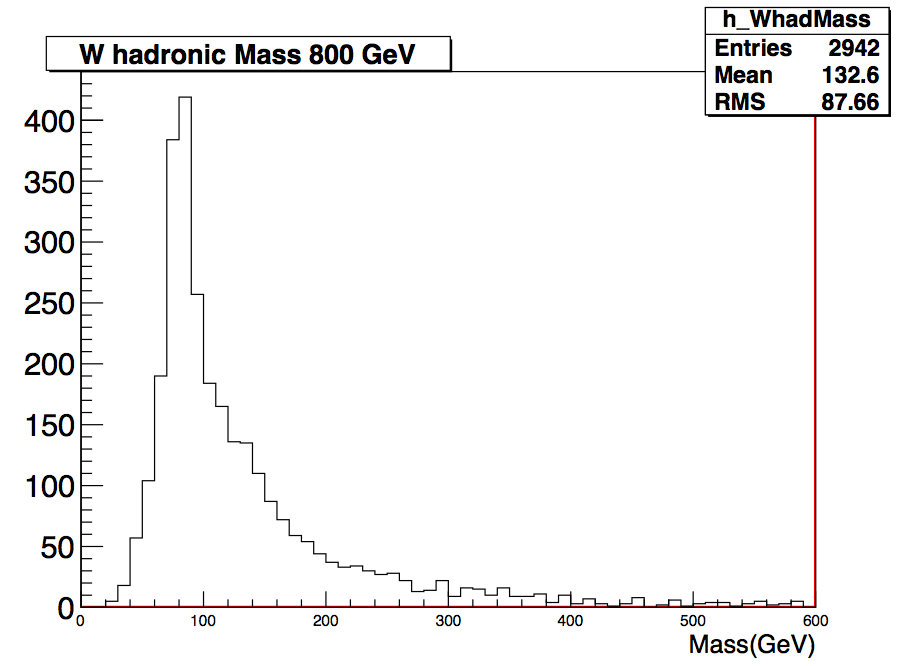
\includegraphics[width=0.8\textwidth]{Whad}
    \caption{\label{Whad} Invariant mass distribution of hadronic $W$ boson assuming there is a signal at 800 $GeV/c^2$.}
\end{figure}     

\begin{figure}[!h]
\centering
    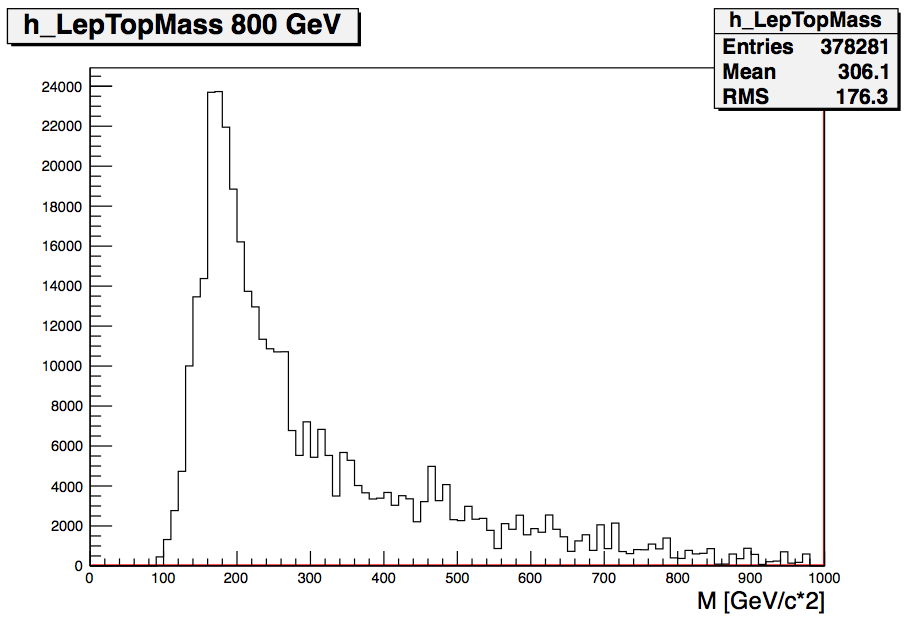
\includegraphics[width=0.8\textwidth]{toplep}
    \caption{\label{toplep} Invariant mass distribution of leptonic top quark assuming there is a signal at 800 $GeV/c^2$.}
\end{figure}

\begin{figure}[!h]
\centering
    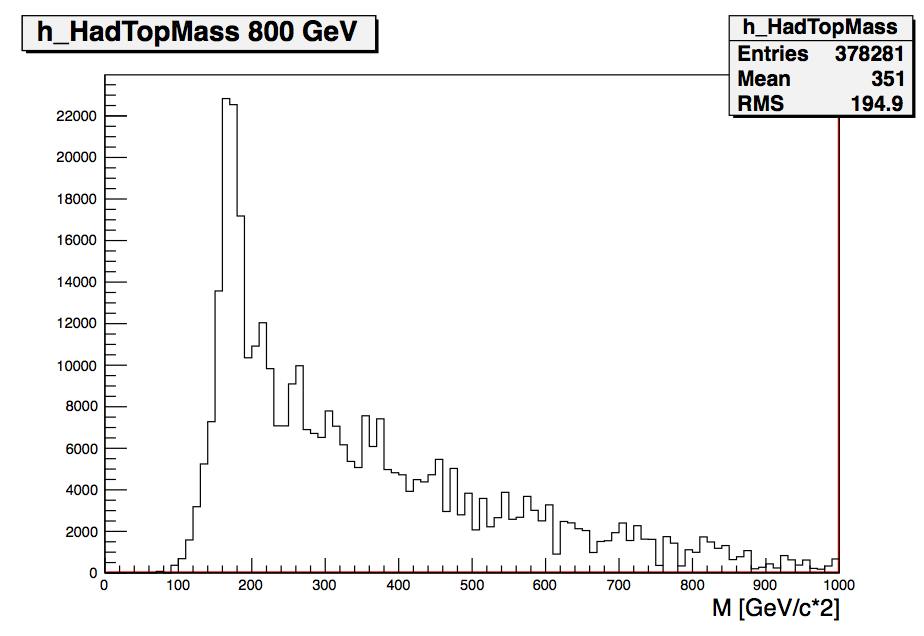
\includegraphics[width=0.8\textwidth]{tophad}
    \caption{\label{tophad} Invariant mass distribution of hadronic top quark assuming there is a signal at 800 $GeV/c^2$.}
\end{figure}

\begin{figure}[!h]
\centering
    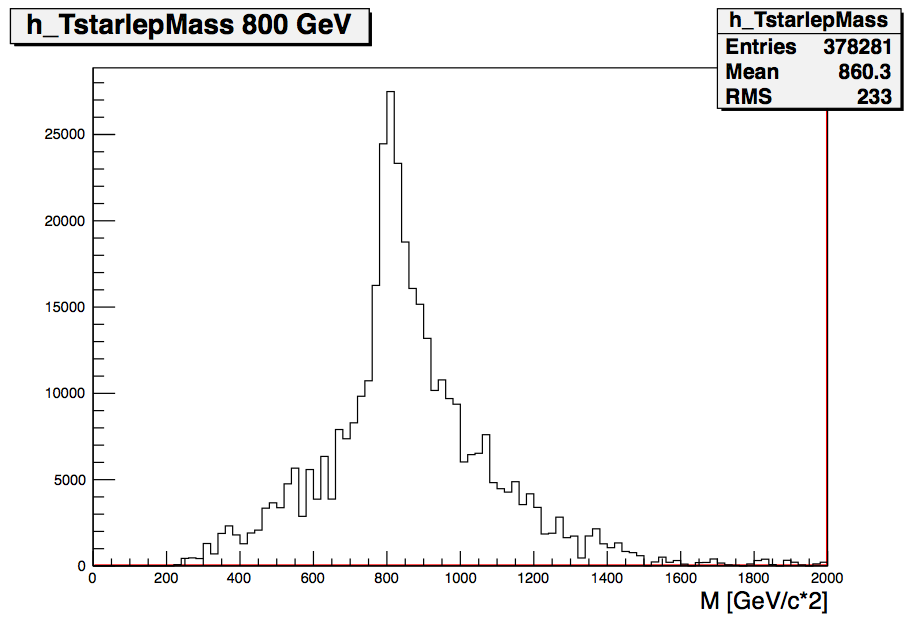
\includegraphics[width=0.8\textwidth]{tstarlep}
    \caption{\label{tstarlep} Invariant mass distribution of leptonic $t^*$  assuming there is a signal at 800 $GeV/c^2$.}
\end{figure}

\begin{figure}[!h]
\centering
    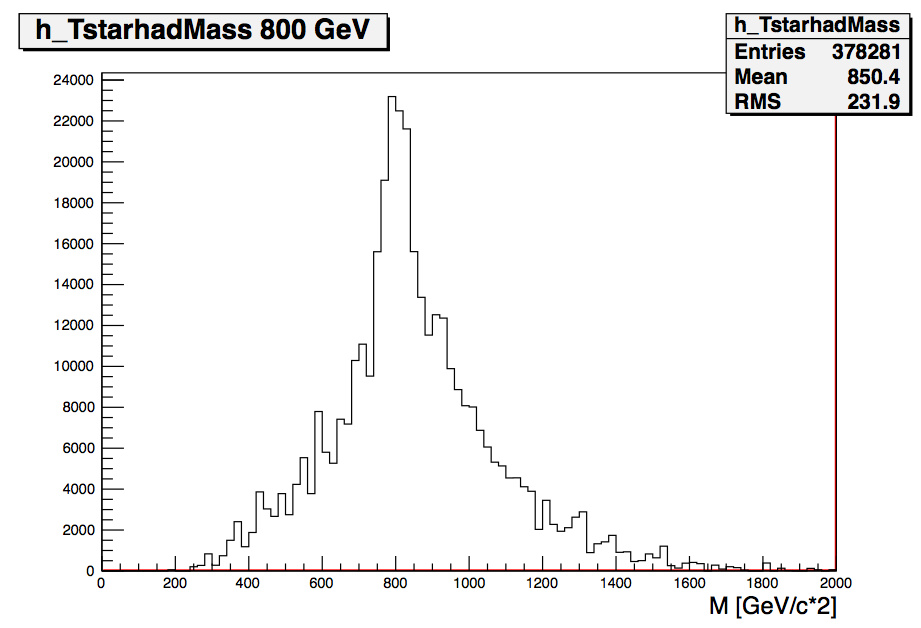
\includegraphics[width=0.8\textwidth]{tstarhad}
    \caption{\label{tstarhad} Invariant mass distribution of hadronic $t^*$  assuming there is a signal at 800 $GeV/c^2$.}
\end{figure}




\section{Fake rate calculation and Background estimation}

The Matrix Method is originally used to determine isolation efficiency of lepton to estimate high-purity QCD multijet beckground from data from a low missing transeverse energy signal region in  $D \emptyset$ experiment at Fermilab.

Nowadays, the so called matrix method is in use for signatures which have two leptons in the final state. Generally matrix method is based on to solve linear system of equations consists of the background and signal components (unknowns),  the yields three levels of selection (knowns) and coefficients of object fake rates and signal efficiencies. The three selection mentioned here stand for loose, medium and tight selection criterias.

This section is dedicated to explain adaption of the matrix method to CMS and diphoton channel by showing detailed calculations of fake rates, efficiencies and their usage. 

\subsection{Matrix Method for Diphoton Channel}

In this analysis, matrix method for diphoton channel cannot be simply applied because there are three sources of fake photons:  fake photons from quarks, from gluons and fake photons from leptons. In total as matrix elements there are two photons can be both fake, both real, or one fake one real aplied loose, medium, tight selections. Thus, the linear system of equation (the matrix) with 18 element can be expressed as in the equations \ref{mm1_}, \ref{mm2_}, \ref{mm3_}.


\begin{eqnarray}
N_{L} & = & \left( N_{L}^{lq} + N_{L}^{lg} + N_{L}^{ll} + N_{L}^{qq} + N_{L}^{gg} + N_{L}^{qg} \right)  \nonumber \\
& & + \left( N_{L}^{sq} + N_{L}^{sg} + N_{L}^{sl} \right) + N_{L}^{ss} \label{mm1_} \\
N_{M} & = & \left( N_{M}^{lq} + N_{M}^{lg} + N_{M}^{ll} + N_{M}^{qq} + N_{M}^{gg} + N_{M}^{qg} \right)  \nonumber \\
& & + \left( N_{M}^{sq} + N_{M}^{sg} + N_{M}^{sl} \right) + N_{M}^{ss} \label{mm2_} \\
N_{T} & = & \left( N_{T}^{lq} + N_{T}^{lg} + N_{T}^{ll} + N_{T}^{qq} + N_{T}^{gg} + N_{T}^{qg} \right)  \nonumber \\
& & + \left( N_{T}^{sq} + N_{T}^{sg} + N_{T}^{sl} \right) + N_{T}^{ss} \label{mm3_}
\end{eqnarray}

In these equations, $l$ indicates the fake photons from leptons, $q$ and $g$ indicates the fake photons from quarks and gluons, respectively, and $s$ stands for the real (signal) photons. Therefore for instance $N_{M}^{lq}$ will be the number of events selected by the medium isolation which have one fake photon from lepton and one fake photon from quark in the final state, while $N_{T}^{sg}$ will be the number of tightly selected events with one real and one fake from gluon final state photon. These equations can be categorized with respect to be fake or real and selected as loose, medium, tight. Equations \ref{eq:N1_}, \ref{eq:N2_}, \ref{eq:eps1_}, \ref{eq:eps2_}, \ref{eq:eps3_}, show definitions yield after this catogarization.

\begin{eqnarray}
N_{L(M)(T)}^{ff} & \equiv & N_{L(M)(T)}^{lq} + N_{L(M)(T)}^{lg} + N_{L(M)(T)}^{ll} \nonumber \\
& & + N_{L(M)(T)}^{qq} + N_{L(M)(T)}^{gg} + N_{L(M)(T)}^{qg}, \label{eq:N1_}\\
N_{L(M)(T)}^{sf} & \equiv & N_{L(M)(T)}^{sq} + N_{L(M)(T)}^{sg} + N_{L(M)(T)}^{sl}. \label{eq:N2_}
\end{eqnarray}

\begin{eqnarray}
\epsilon_{ff}^{L \rightarrow M(T)} & \equiv & \frac{N_{M(T)}^{ff}}{N_{L}^{ff}}, \label{eq:eps1_}\\
\epsilon_{sf}^{L \rightarrow M(T)} & \equiv & \frac{N_{M(T)}^{sf}}{N_{L}^{sf}}, \label{eq:eps2_}\\
\epsilon_{ss}^{L \rightarrow M(T)} & \equiv & \frac{N_{M(T)}^{ss}}{N_{L}^{ss}}. \label{eq:eps3_}
\end{eqnarray}

Thus, when these definitions put in to equations \ref{mm1_}, \ref{mm2_}, \ref{mm3_}, the system of equations can be rewritted as:

\begin{eqnarray}
N_{L} & = & N_{L}^{ff} + N_{L}^{sf} + N_{L}^{ss}, \label{eq:mm4_}\\
N_{M} & = & \epsilon_{ff}^{L \rightarrow M} N_{L}^{ff} + \epsilon_{sf}^{L \rightarrow M} N_{L}^{sf} + \epsilon_{ss}^{L \rightarrow M} N_{L}^{ss}, \label{eq:mm5_}\\
N_{T} & = & \epsilon_{ff}^{L \rightarrow T} N_{L}^{ff} + \epsilon_{sf}^{L \rightarrow T} N_{L}^{sf} + \epsilon_{ss}^{L \rightarrow T} N_{L}^{ss}. \label{eq:mm6_}
\end{eqnarray}

%%%%%
%%%%%
%%%%%
%%%%%

And the components of the $\epsilon$s:

\begin{eqnarray}
\epsilon_{lq}^{L \rightarrow M(T)} & \equiv & \frac{N_{M(T)}^{lq}}{N_{L}^{ff}}, \label{eq:eps4_}\\
\epsilon_{lg}^{L \rightarrow M(T)} & \equiv & \frac{N_{M(T)}^{lg}}{N_{L}^{ff}}, \label{eq:eps4__}\\
\epsilon_{ll}^{L \rightarrow M(T)} & \equiv & \frac{N_{M(T)}^{ll}}{N_{L}^{ff}}, \label{eq:eps5_}\\
\epsilon_{qq}^{L \rightarrow M(T)} & \equiv & \frac{N_{M(T)}^{qq}}{N_{L}^{ff}}, \label{eq:eps6__}\\
\epsilon_{gg}^{L \rightarrow M(T)} & \equiv & \frac{N_{M(T)}^{gg}}{N_{L}^{ff}}, \label{eq:eps6___}\\
\epsilon_{qg}^{L \rightarrow M(T)} & \equiv & \frac{N_{M(T)}^{qg}}{N_{L}^{ff}}, \label{eq:eps6____}\\
\epsilon_{sq}^{L \rightarrow M(T)} & \equiv & \frac{N_{M(T)}^{sq}}{N_{L}^{sf}}, \label{eq:eps7}\\
\epsilon_{sg}^{L \rightarrow M(T)} & \equiv & \frac{N_{M(T)}^{sg}}{N_{L}^{sf}}, \label{eq:eps8}\\
\epsilon_{sl}^{L \rightarrow M(T)} & \equiv & \frac{N_{M(T)}^{sl}}{N_{L}^{sf}}. \label{eq:eps8_}
\end{eqnarray}

Since $\epsilon$s are linearly independent coefficiants can be written:

\begin{eqnarray}
\epsilon_{ff}^{L \rightarrow M(T)} & = & \epsilon_{lq}^{L \rightarrow M(T)} + \epsilon_{lg}^{L \rightarrow M(T)} + \epsilon_{ll}^{L \rightarrow M(T)} \nonumber \\
& & + \epsilon_{qq}^{L \rightarrow M(T)} + \epsilon_{gg}^{L \rightarrow M(T)} + \epsilon_{qg}^{L \rightarrow M(T)} \label{eq:eps9_} \\ 
\epsilon_{sf}^{L \rightarrow M(T)} & = & \epsilon_{sq}^{L \rightarrow M(T)} + \epsilon_{sg}^{L \rightarrow M(T)} + \epsilon_{sl}^{L \rightarrow M(T)} \label{eq:eps10_}
\end{eqnarray}

In order to define elements can be estimated from data, the following calculations are necessary. 

\begin{eqnarray}
\epsilon_{lq}^{L \rightarrow T} & = & \frac{N_{T}^{lq}}{N_{L}^{lq}+N_{L}^{lg}+N_{L}^{ll}+N_{L}^{qq}+N_{L}^{gg}+N_{L}^{qg}} \nonumber \\ 
& = &
\frac{N_{T}^{lq}}{N_{L}^{lq}} \cdot \frac{1}{1 + \frac{N_{L}^{lg}}{N_{L}^{lq}} + \frac{N_{L}^{ll}}{N_{L}^{lq}} + \frac{N_{L}^{qq}}{N_{L}^{lq}} + \frac{N_{L}^{gg}}{N_{L}^{lq}} + \frac{N_{L}^{qg}}{N_{L}^{lq}}} \nonumber \\
& = & \epsilon_{l} \epsilon_{q} \cdot \frac{1}{1 + R^{lg/lq} + R^{ll/lq} + R^{qq/lq} + R^{gg/lq} + R^{qg/lq}} \label{eq:eps11_}\\
\epsilon_{lg}^{L \rightarrow T} & = & \frac{N_{T}^{lg}}{N_{L}^{lq}+N_{L}^{lg}+N_{L}^{ll}+N_{L}^{qq}+N_{L}^{gg}+N_{L}^{qg}} \nonumber \\
& = &
\frac{N_{T}^{lg}}{N_{L}^{lg}} \cdot \frac{1}{1 + \frac{N_{L}^{lq}}{N_{L}^{lg}} + \frac{N_{L}^{ll}}{N_{L}^{lg}} + \frac{N_{L}^{qq}}{N_{L}^{lg}} + \frac{N_{L}^{gg}}{N_{L}^{lg}} + \frac{N_{L}^{qg}}{N_{L}^{lg}}} \nonumber \\
& = & \epsilon_{l} \epsilon_{g} \cdot \frac{1}{1 + R^{lq/lg} + R^{ll/lg} + R^{qq/lg} + R^{gg/lg} + R^{qg/lg}} \label{eq:eps12_}\\
\epsilon_{ll}^{L \rightarrow T} & = & \frac{N_{T}^{ll}}{N_{L}^{lq}+N_{L}^{lg}+N_{L}^{ll}+N_{L}^{qq}+N_{L}^{gg}+N_{L}^{qg}} \nonumber \\
& = &
\frac{N_{T}^{ll}}{N_{L}^{ll}} \cdot \frac{1}{1 + \frac{N_{L}^{lq}}{N_{L}^{ll}} + \frac{N_{L}^{lg}}{N_{L}^{ll}} + \frac{N_{L}^{qq}}{N_{L}^{ll}} + \frac{N_{L}^{gg}}{N_{L}^{ll}} + \frac{N_{L}^{qg}}{N_{L}^{ll}}} \nonumber \\
& = & \epsilon_{l}^{2} \cdot \frac{1}{1 + R^{lq/ll} + R^{lg/ll} + R^{qq/ll} + R^{gg/ll} + R^{qg/ll}}, \label{eq:eps13_}\\
\epsilon_{qq}^{L \rightarrow T} & = & \frac{N_{T}^{qq}}{N_{L}^{lq}+N_{L}^{lg}+N_{L}^{ll}+N_{L}^{qq}+N_{L}^{gg}+N_{L}^{qg}} \nonumber \\
& = &  
\frac{N_{T}^{qq}}{N_{L}^{qq}} \cdot \frac{1}{1 + \frac{N_{L}^{lq}}{N_{L}^{qq}} + \frac{N_{L}^{lg}}{N_{L}^{qq}} + \frac{N_{L}^{ll}}{N_{L}^{qq}} + \frac{N_{L}^{gg}}{N_{L}^{qq}} + \frac{N_{L}^{qg}}{N_{L}^{qq}}} \nonumber \\
& = & \epsilon_{q}^{2} \cdot \frac{1}{1 + R^{lq/qq} + R^{lg/qq} + R^{ll/qq} + R^{gg/qq} + R^{qg/qq}} \label{eq:eps14_}\\
\epsilon_{gg}^{L \rightarrow T} & = & \frac{N_{T}^{gg}}{N_{L}^{lq}+N_{L}^{lg}+N_{L}^{ll}+N_{L}^{qq}+N_{L}^{gg}+N_{L}^{qg}} \nonumber \\
& = & 
\frac{N_{T}^{gg}}{N_{L}^{gg}} \cdot \frac{1}{1 + \frac{N_{L}^{lq}}{N_{L}^{gg}} + \frac{N_{L}^{lg}}{N_{L}^{gg}} + \frac{N_{L}^{ll}}{N_{L}^{gg}} + \frac{N_{L}^{qq}}{N_{L}^{gg}} + \frac{N_{L}^{qg}}{N_{L}^{gg}}} \nonumber \\
& = & \epsilon_{g}^{2} \cdot \frac{1}{1 + R^{lq/gg} + R^{lg/gg} + R^{ll/gg} + R^{qq/gg} + R^{qg/gg}} \label{eq:eps15_}\\
\epsilon_{qg}^{L \rightarrow T} & = & \frac{N_{T}^{qg}}{N_{L}^{lq}+N_{L}^{lg}+N_{L}^{ll}+N_{L}^{qq}+N_{L}^{gg}+N_{L}^{qg}} \nonumber \\
& = & 
\frac{N_{T}^{qg}}{N_{L}^{qg}} \cdot \frac{1}{1 + \frac{N_{L}^{lq}}{N_{L}^{qg}} + \frac{N_{L}^{lg}}{N_{L}^{qg}} + \frac{N_{L}^{ll}}{N_{L}^{qg}} + \frac{N_{L}^{qq}}{N_{L}^{qg}} + \frac{N_{L}^{gg}}{N_{L}^{qg}}} \nonumber \\
& = & \epsilon_{q} \epsilon_{g} \cdot \frac{1}{1 + R^{lq/qg} + R^{lg/qg} + R^{ll/qg} + R^{qq/qg} + R^{gg/qg}} \label{eq:eps16_}
\end{eqnarray}

\begin{eqnarray}
\epsilon_{lq}^{L \rightarrow M} & = & \frac{N_{M}^{lq}}{N_{L}^{lq}+N_{L}^{lg}+N_{L}^{ll}+N_{L}^{qq}+N_{L}^{gg}+N_{L}^{qg}} \nonumber \\
& = & 
\frac{N_{M}^{lq}}{N_{L}^{lq}} \cdot \frac{1}{1 + \frac{N_{L}^{lg}}{N_{L}^{lq}} + \frac{N_{L}^{ll}}{N_{L}^{lq}} + \frac{N_{L}^{qq}}{N_{L}^{lq}} + \frac{N_{L}^{gg}}{N_{L}^{lq}} + \frac{N_{L}^{qg}}{N_{L}^{lq}}} \nonumber \\
& = & \left( \epsilon_{l} + \epsilon_{q} - \epsilon_{l} \epsilon_{q} \right) \cdot \frac{1}{1 + R^{lg/lq} + R^{ll/lq} + R^{qq/lq} + R^{gg/lq} + R^{qg/lq}} \label{eq:eps11_}\\
\epsilon_{lg}^{L \rightarrow M} & = & \frac{N_{M}^{lg}}{N_{L}^{lq}+N_{L}^{lg}+N_{L}^{ll}+N_{L}^{qq}+N_{L}^{gg}+N_{L}^{qg}} \nonumber \\
& = & 
\frac{N_{M}^{lg}}{N_{L}^{lg}} \cdot \frac{1}{1 + \frac{N_{L}^{lq}}{N_{L}^{lg}} + \frac{N_{L}^{ll}}{N_{L}^{lg}} + \frac{N_{L}^{qq}}{N_{L}^{lg}} + \frac{N_{L}^{gg}}{N_{L}^{lg}} + \frac{N_{L}^{qg}}{N_{L}^{lg}}} \nonumber \\
& = & \left( \epsilon_{l} + \epsilon_{g} - \epsilon_{l} \epsilon_{g} \right) \cdot \frac{1}{1 + R^{lq/lg} + R^{ll/lg} + R^{qq/lg} + R^{gg/lg} + R^{qg/lg}} \label{eq:eps12__}\\
\epsilon_{ll}^{L \rightarrow M} & = & \frac{N_{M}^{ll}}{N_{L}^{lq}+N_{L}^{lg}+N_{L}^{ll}+N_{L}^{qq}+N_{L}^{gg}+N_{L}^{qg}} \nonumber \\
& = & 
\frac{N_{M}^{ll}}{N_{L}^{ll}} \cdot \frac{1}{1 + \frac{N_{L}^{lq}}{N_{L}^{ll}} + \frac{N_{L}^{lg}}{N_{L}^{ll}} + \frac{N_{L}^{qq}}{N_{L}^{ll}} + \frac{N_{L}^{gg}}{N_{L}^{ll}} + \frac{N_{L}^{qg}}{N_{L}^{ll}}} \nonumber \\
& = & \left( 2 \epsilon_{l} - \epsilon_{l}^{2} \right) \cdot \frac{1}{1 + R^{lq/ll} + R^{lg/ll} + R^{qq/ll} + R^{gg/ll} + R^{qg/ll}} \label{eq:eps13__}\\
\epsilon_{qq}^{L \rightarrow M} & = & \frac{N_{M}^{qq}}{N_{L}^{lq}+N_{L}^{lg}+N_{L}^{ll}+N_{L}^{qq}+N_{L}^{gg}+N_{L}^{qg}} \nonumber \\
& = &
\frac{N_{M}^{qq}}{N_{L}^{qq}} \cdot \frac{1}{1 + \frac{N_{L}^{lq}}{N_{L}^{qq}} + \frac{N_{L}^{lg}}{N_{L}^{qq}} + \frac{N_{L}^{ll}}{N_{L}^{qq}} + \frac{N_{L}^{gg}}{N_{L}^{qq}} + \frac{N_{L}^{qg}}{N_{L}^{qq}}} \nonumber \\
& = & \left( 2 \epsilon_{q} - \epsilon_{q}^{2} \right) \cdot \frac{1}{1 + R^{lq/qq} + R^{lg/qq} + R^{ll/qq} + R^{gg/qq} + R^{qg/qq}} \label{eq:eps14__}\\
\epsilon_{gg}^{L \rightarrow M} & = & \frac{N_{M}^{gg}}{N_{L}^{lq}+N_{L}^{lg}+N_{L}^{ll}+N_{L}^{qq}+N_{L}^{gg}+N_{L}^{qg}} \nonumber \\
& = &
\frac{N_{M}^{gg}}{N_{L}^{gg}} \cdot \frac{1}{1 + \frac{N_{L}^{lq}}{N_{L}^{gg}} + \frac{N_{L}^{lg}}{N_{L}^{gg}} + \frac{N_{L}^{ll}}{N_{L}^{gg}} + \frac{N_{L}^{qq}}{N_{L}^{gg}} + \frac{N_{L}^{qg}}{N_{L}^{gg}}} \nonumber \\
& = & \left( 2 \epsilon_{g} - \epsilon_{g}^{2} \right) \cdot \frac{1}{1 + R^{lq/gg} + R^{lg/gg} + R^{ll/gg} + R^{qq/gg} + R^{qg/gg}} \label{eq:eps15__}\\
\epsilon_{qg}^{L \rightarrow M} & = & \frac{N_{M}^{qg}}{N_{L}^{lq}+N_{L}^{lg}+N_{L}^{ll}+N_{L}^{qq}+N_{L}^{gg}+N_{L}^{qg}} \nonumber \\
& = &
\frac{N_{M}^{qg}}{N_{L}^{qg}} \cdot \frac{1}{1 + \frac{N_{L}^{lq}}{N_{L}^{qg}} + \frac{N_{L}^{lg}}{N_{L}^{qg}} + \frac{N_{L}^{ll}}{N_{L}^{qg}} + \frac{N_{L}^{qq}}{N_{L}^{qg}} + \frac{N_{L}^{gg}}{N_{L}^{qg}}} \nonumber \\
& = & \left( \epsilon_{q} + \epsilon_{g} - \epsilon_{q} \epsilon_{g} \right) \cdot \frac{1}{1 + R^{lq/qg} + R^{lg/qg} + R^{ll/qg} + R^{qq/qg} + R^{gg/qg}} \label{eq:eps16__}
\end{eqnarray}

\begin{eqnarray}
\epsilon_{sq}^{L \rightarrow T} & = & \frac{N_{T}^{sq}}{N_{L}^{sq}+N_{L}^{sg}+N_{L}^{sl}} = \frac{N_{T}^{sq}}{N_{L}^{sq}} \cdot \frac{1}{1 + \frac{N_{L}^{sg}}{N_{L}^{sq}} + \frac{N_{L}^{sl}}{N_{L}^{sq}}} \nonumber \\
& = & \epsilon_{s} \epsilon_{q} \cdot \frac{1}{1 + R^{sg/sq} + R^{sl/sq}}, \label{eq:eps17_}\\
\epsilon_{sg}^{L \rightarrow T} & = & \frac{N_{T}^{sg}}{N_{L}^{sq}+N_{L}^{sg}+N_{L}^{sl}} = \frac{N_{T}^{sg}}{N_{L}^{sg}} \cdot \frac{1}{1 + \frac{N_{L}^{sq}}{N_{L}^{sg}} + \frac{N_{L}^{sl}}{N_{L}^{sg}}} \nonumber \\
& = & \epsilon_{s} \epsilon_{g} \cdot \frac{1}{1 + R^{sq/sg} + R^{sl/sg}}, \label{eq:eps17__}\\
\epsilon_{sl}^{L \rightarrow T} & = & \frac{N_{T}^{sl}}{N_{L}^{sq}+N_{L}^{sg}+N_{L}^{sl}} = \frac{N_{T}^{sl}}{N_{L}^{sl}} \cdot \frac{1}{1 + \frac{N_{L}^{sq}}{N_{L}^{sl}} + \frac{N_{L}^{sg}}{N_{L}^{sl}}} \nonumber \\
& = & \epsilon_{s} \epsilon_{l} \cdot \frac{1}{1 + R^{sq/sl} + R^{sg/sl}}, \label{eq:eps17___}\\
\epsilon_{sq}^{L \rightarrow M} & = & \frac{N_{M}^{sq}}{N_{L}^{sq}+N_{L}^{sg}+N_{L}^{sl}} = \frac{N_{M}^{sq}}{N_{L}^{sq}} \cdot \frac{1}{1 + \frac{N_{L}^{sg}}{N_{L}^{sq}} + \frac{N_{L}^{sl}}{N_{L}^{sq}}} \nonumber \\
& = & \left( \epsilon_{s} + \epsilon_{q} - \epsilon_{s} \epsilon_{q} \right) \cdot \frac{1}{1 + R^{sg/sq} + R^{sl/sq}}, \label{eq:eps18_}\\
\epsilon_{sg}^{L \rightarrow M} & = & \frac{N_{M}^{sg}}{N_{L}^{sq}+N_{L}^{sg}+N_{L}^{sl}} = \frac{N_{M}^{sg}}{N_{L}^{sg}} \cdot \frac{1}{1 + \frac{N_{L}^{sq}}{N_{L}^{sg}} + \frac{N_{L}^{sl}}{N_{L}^{sg}}} \nonumber \\
& = & \left( \epsilon_{s} + \epsilon_{g} - \epsilon_{s} \epsilon_{g} \right) \cdot \frac{1}{1 + R^{sq/sg} + R^{sl/sg}}, \label{eq:eps18__}\\
\epsilon_{sl}^{L \rightarrow M} & = & \frac{N_{M}^{sl}}{N_{L}^{sq}+N_{L}^{sg}+N_{L}^{sl}} = \frac{N_{M}^{sl}}{N_{L}^{sl}} \cdot \frac{1}{1 + \frac{N_{L}^{sq}}{N_{L}^{sl}} + \frac{N_{L}^{sg}}{N_{L}^{sl}}} \nonumber \\
& = & \left( \epsilon_{s} + \epsilon_{l} - \epsilon_{s} \epsilon_{l} \right) \cdot \frac{1}{1 + R^{sq/sl} + R^{sg/sl}}, \label{eq:eps18___}\\
\epsilon_{ss}^{L \rightarrow T} & = & \frac{N_{T}^{ss}}{N_{L}^{ss}} = \epsilon_{s}^2, \label{eq:eps21_}\\
\epsilon_{ss}^{L \rightarrow M} & = & \frac{N_{M}^{ss}}{N_{L}^{ss}} = 2 \epsilon_{s} - \epsilon_{s}^2. \label{eq:eps22_}
\end{eqnarray}

where the ratio factors $R^{xy/st}$ are defined as following:


\begin{eqnarray}
R^{xy/st} \equiv \frac{N_{L}^{xy}}{N_{L}^{st}}. \label{eq:R1}
\end{eqnarray}

The system of equations can be solved by estimating the object-level efficiencies ($\epsilon_l$, $\epsilon_q$, $\epsilon_g$, $\epsilon_s$) and the ratio factors from data.

Application of this method to the $t^{*}$ diphoton channel will be discussed in the following subsections.

The efficiency $\epsilon_l$ can be estimated from a Tag and Probe technique on an electron-photon sample, while the efficiency  $\epsilon_q$, $\epsilon_g$ can be estimated with a template fitting procedure on QCD enriched sample. The real photon efficiency $\epsilon_s$ can be calculated again by means of a Tag and Probe technique, by fitting the invariant mass of the di-muon gamma sample. Finally, the ratio factors are estimated by counting the number of two object events in the signal region of the samples. 

The estimation of background events number containing one or two fake photons from data depends on estimation of  the efficiency and ratio factors from data. The following subsections are reserved for describing the procedure of the ratio factors, the fake rate from leptons,  from jets (produced by the hadronization of quark-like and gluon-like partons), and the real photon efficiency estimations from data.

\subsubsection{Photon Fake Rate from leptons}
\label{fakerateleptons}
Initially, it should be noted that $\epsilon$s should be seen as a relative fake rate because they are defined to be a ratio of fake rates (or signal efficiencies).
In the case of the fake rate from leptons, two selections are defined to calculate the ratio: tight selection, no-electron-veto selectio. The tight selection is the usual tight ID photon selection, while the no-electron-veto selection will be the tight ID selection with the exception of the electron-veto cut. Thus, the $\epsilon_{l}$ is defined as the per-object ratio of the photon fake rate for the tight selection over the fake rate for the no-electron-veto selection.


\begin{figure}[!ht]
  \begin{center}
       \resizebox{10cm}{!}{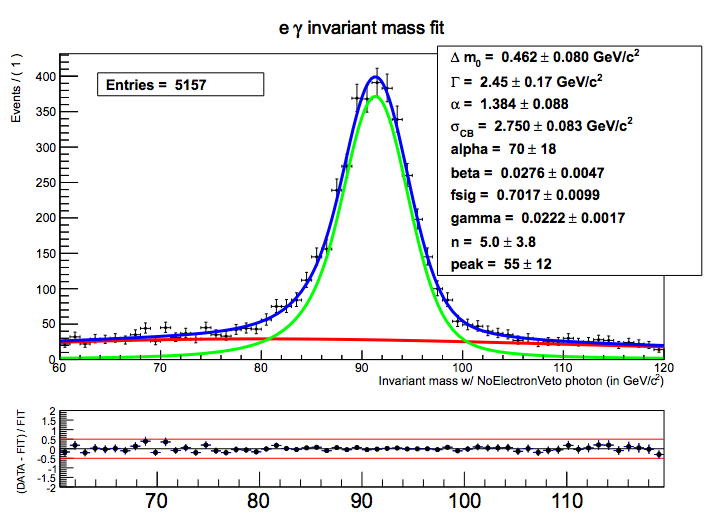
\includegraphics{ResidualDenominator_binned_negligible_errorfit}} 
       \resizebox{10cm}{!}{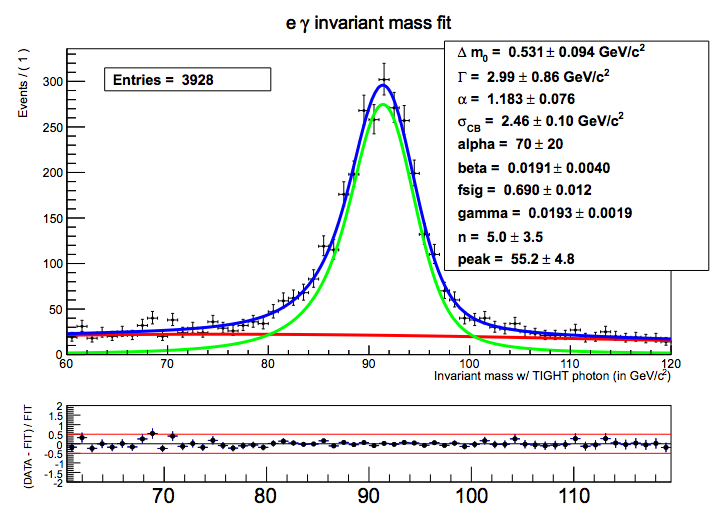
\includegraphics{ResidualNumerator_binned_negligible_errorfit}} 
  \end{center}
    \caption{Electron-Photon invariant mass fit for the no-electron-veto selection (upper plot) and the tight ID selection (lower plot). The fit fuction is a BreitWigner convoluted to a Crystall Ball with a fast Fourier trasformation (for the signal) plus a CMSShape (for the background).}
    \label{Zmass_lepton}
\end{figure}

A Tag and Probe technique, explained at the end of this subsection, is used in order to count the number of fake photons for the tight and no-electron-veto selection. Figure \ref{Zmass_lepton} shows the invariant mass of an electron and a photon fitted with a BreitWigner \cite{R35} convoluted to a Crystall Ball \cite{R35} (for the signal) with a fast Fourier trasformation plus a CMSShape (for the background) where CMSShape can be defined as complementary error function multiplied with an exponential. The implementation of this function can be found in corresponding directory of CMSSW \footnote{/CMSSW/PhysicsTools/TagAndProbe/interface}.
This permits to subtract the non Drell-Yan component. As in the figure, the fit is performed in the invariant mass range between 60 and 120 GeV. The number of fake photons for $\epsilon_{l}$ calculation is the signal event number of these two fitted distributions.

For the object selection for fake photon calculation, electrons passed tight selections and with transverse momenta larger 20 GeV/c are investigated. The transverse momenta cut was 30 GeV/c for the mass reconstruction in sec \ref{elements}, it is lowered to get enough statistics at the low end of the invariant mass distribution. Moreover, the kinematic photon selection and event selection is the same as in the section \ref{elements}. $\eta$, Jet multiplicity, vertex multiplicity and transverse momentum dependencies of $\epsilon_{l}$ can be seen in figures \ref{Feta}, \ref{FJet}, \ref{FNVTX}, \ref{FPT}.

\begin{figure}[!hbt]
\centering
    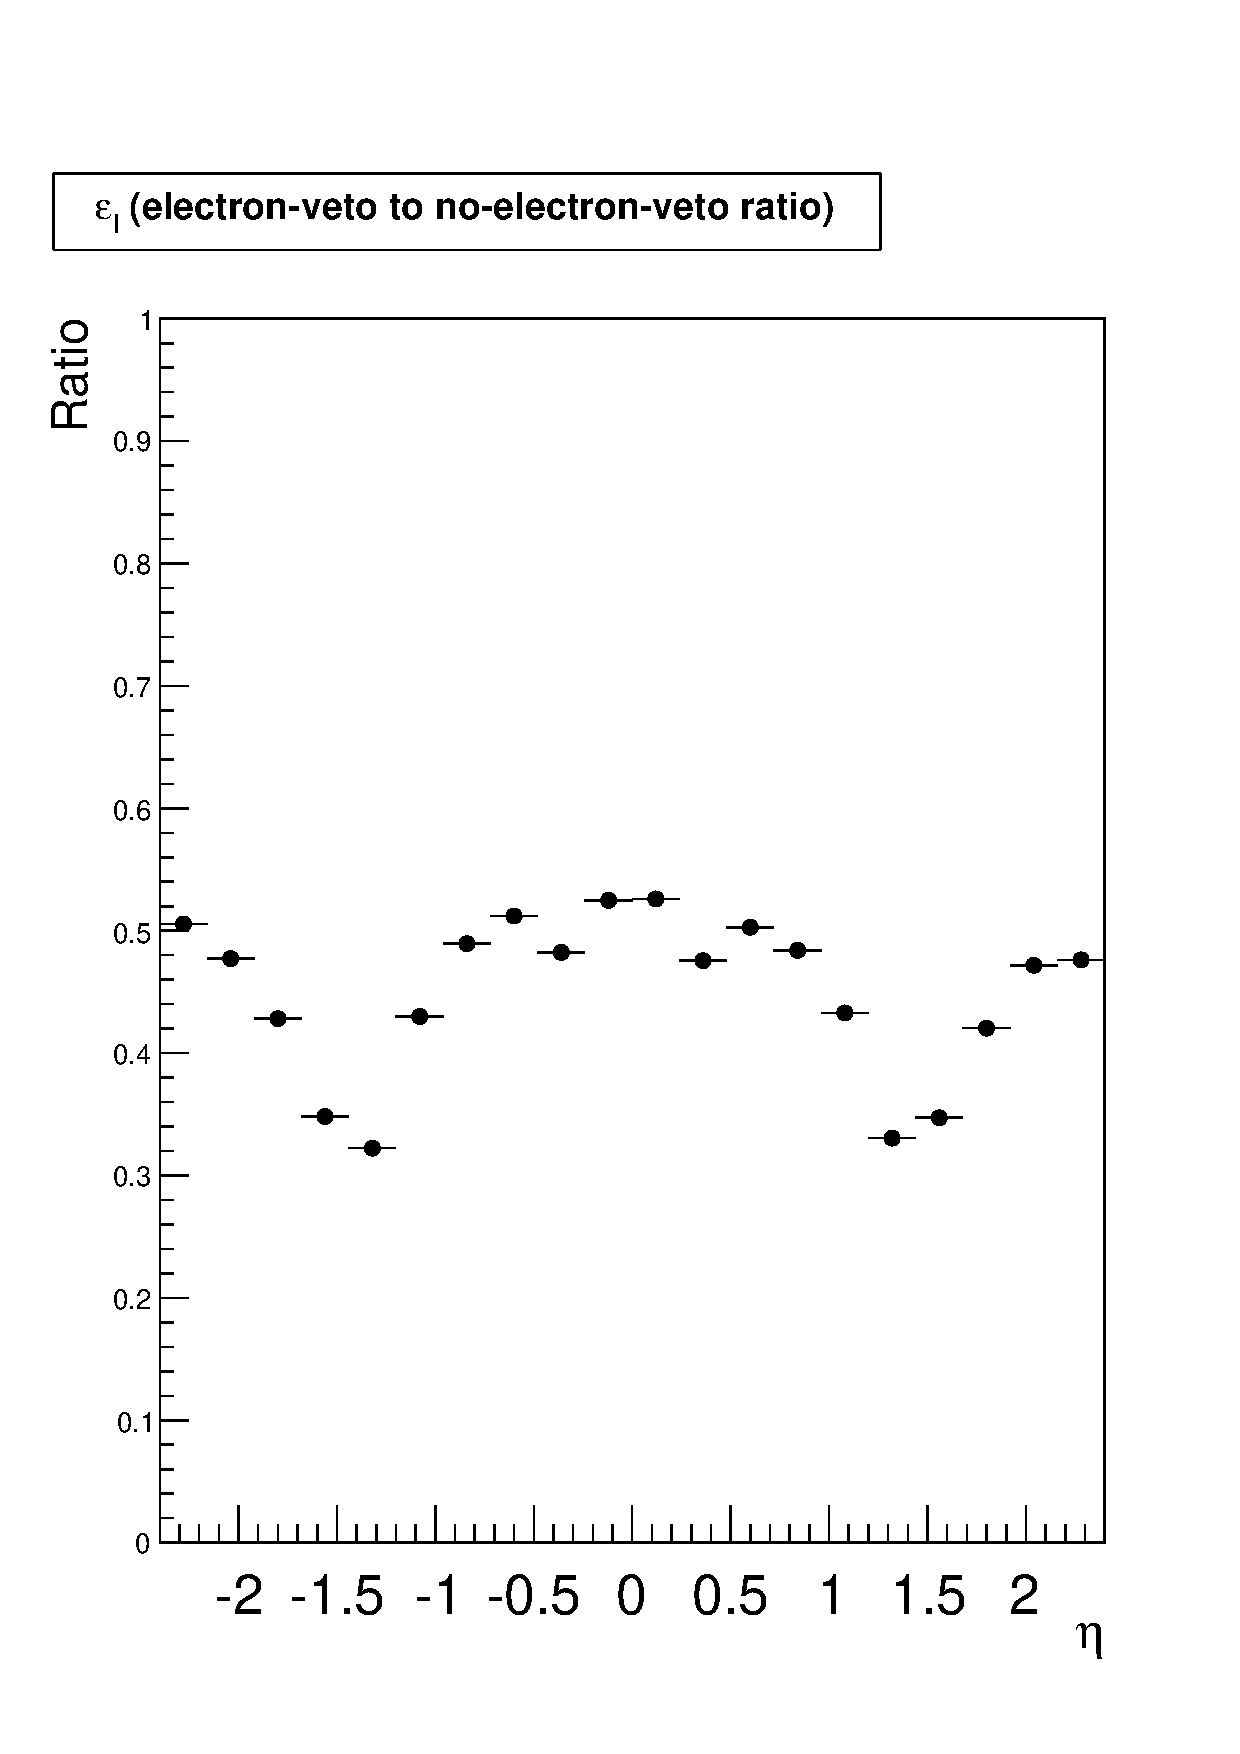
\includegraphics[width=0.8\textwidth]{FakeRateRatio_Eta}
    \caption{\label{Feta} $\epsilon l$: electron-veto to no-electron-veto ratio to Eta .}
\end{figure}

\begin{figure}[!hbt]
\centering
    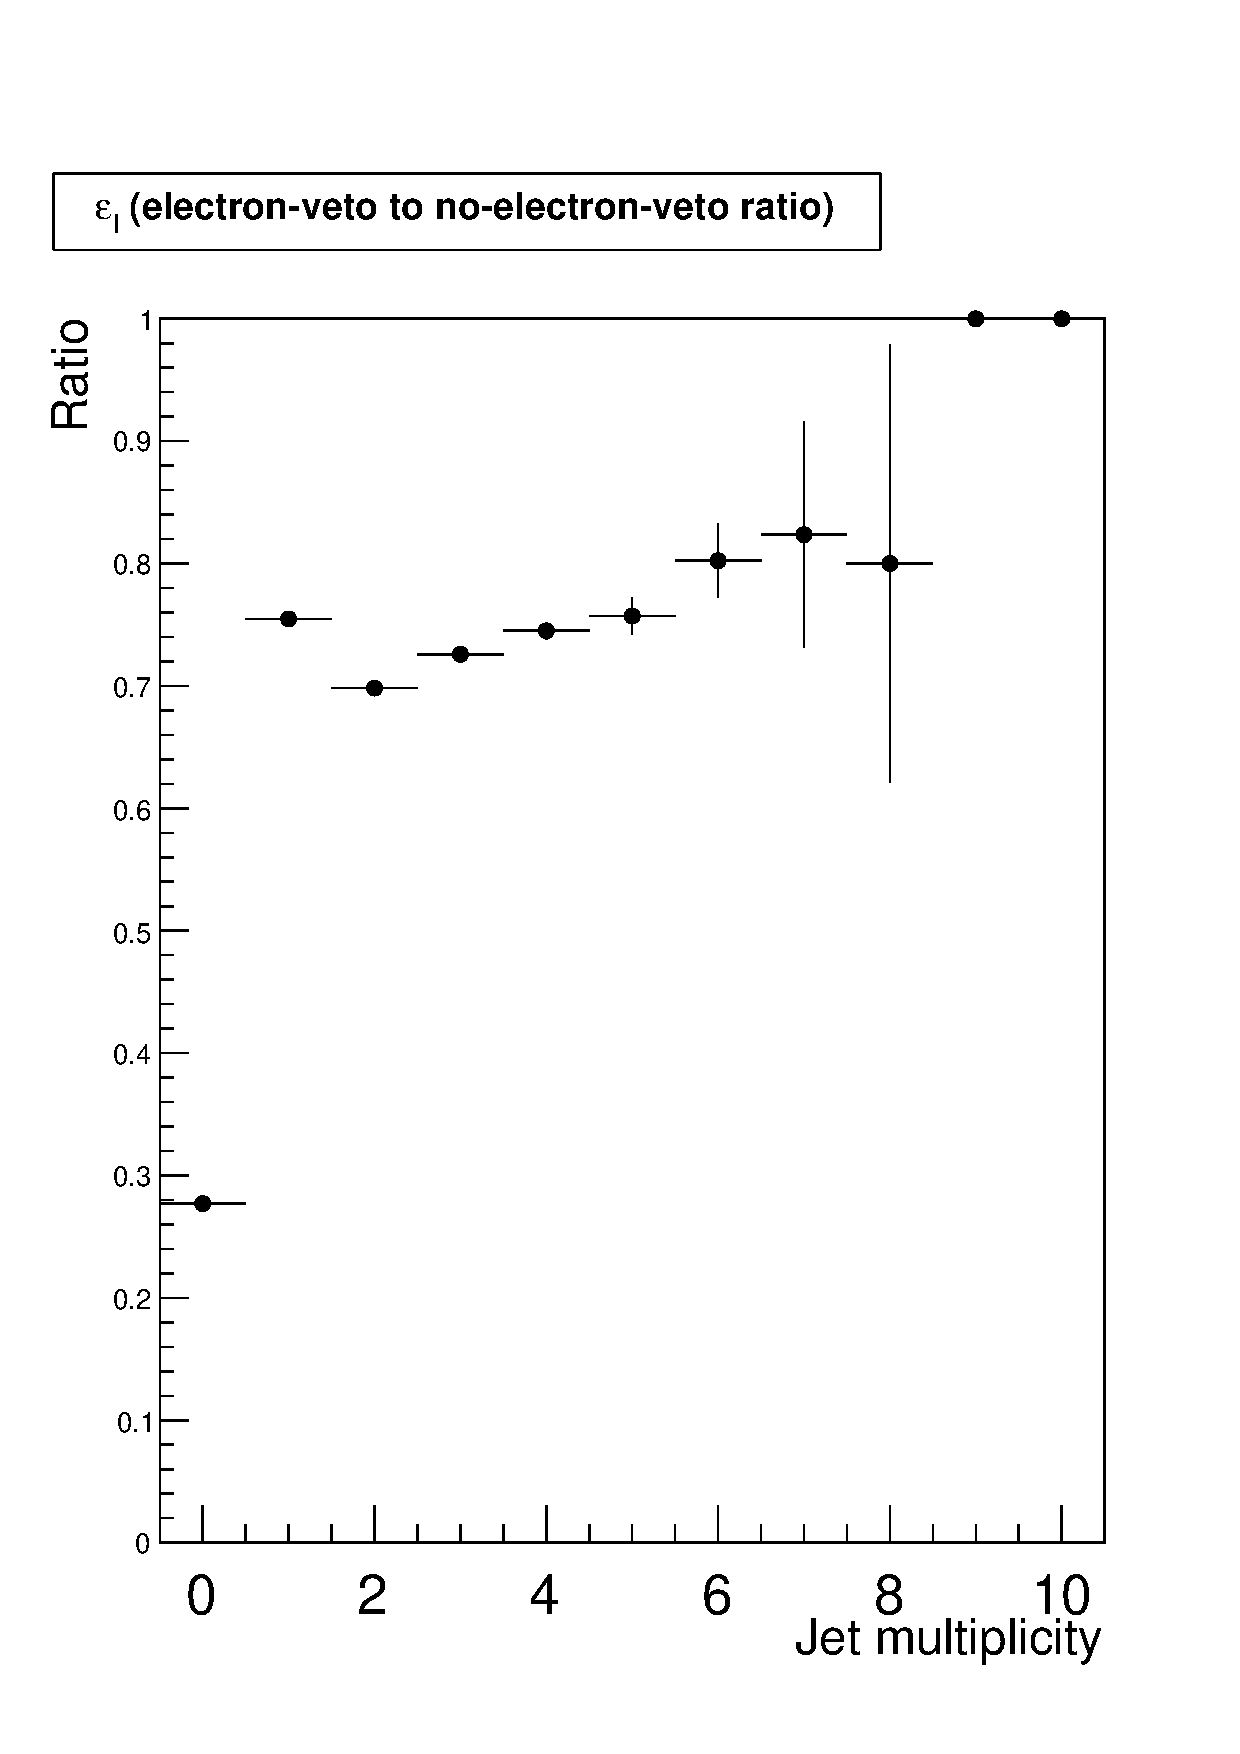
\includegraphics[width=0.8\textwidth]{FakeRateRatio_NJets}
    \caption{\label{FJet} $\epsilon l$: electron-veto to no-electron-veto ratio to NJets .}
\end{figure}

\begin{figure}[!hbt]
\centering
    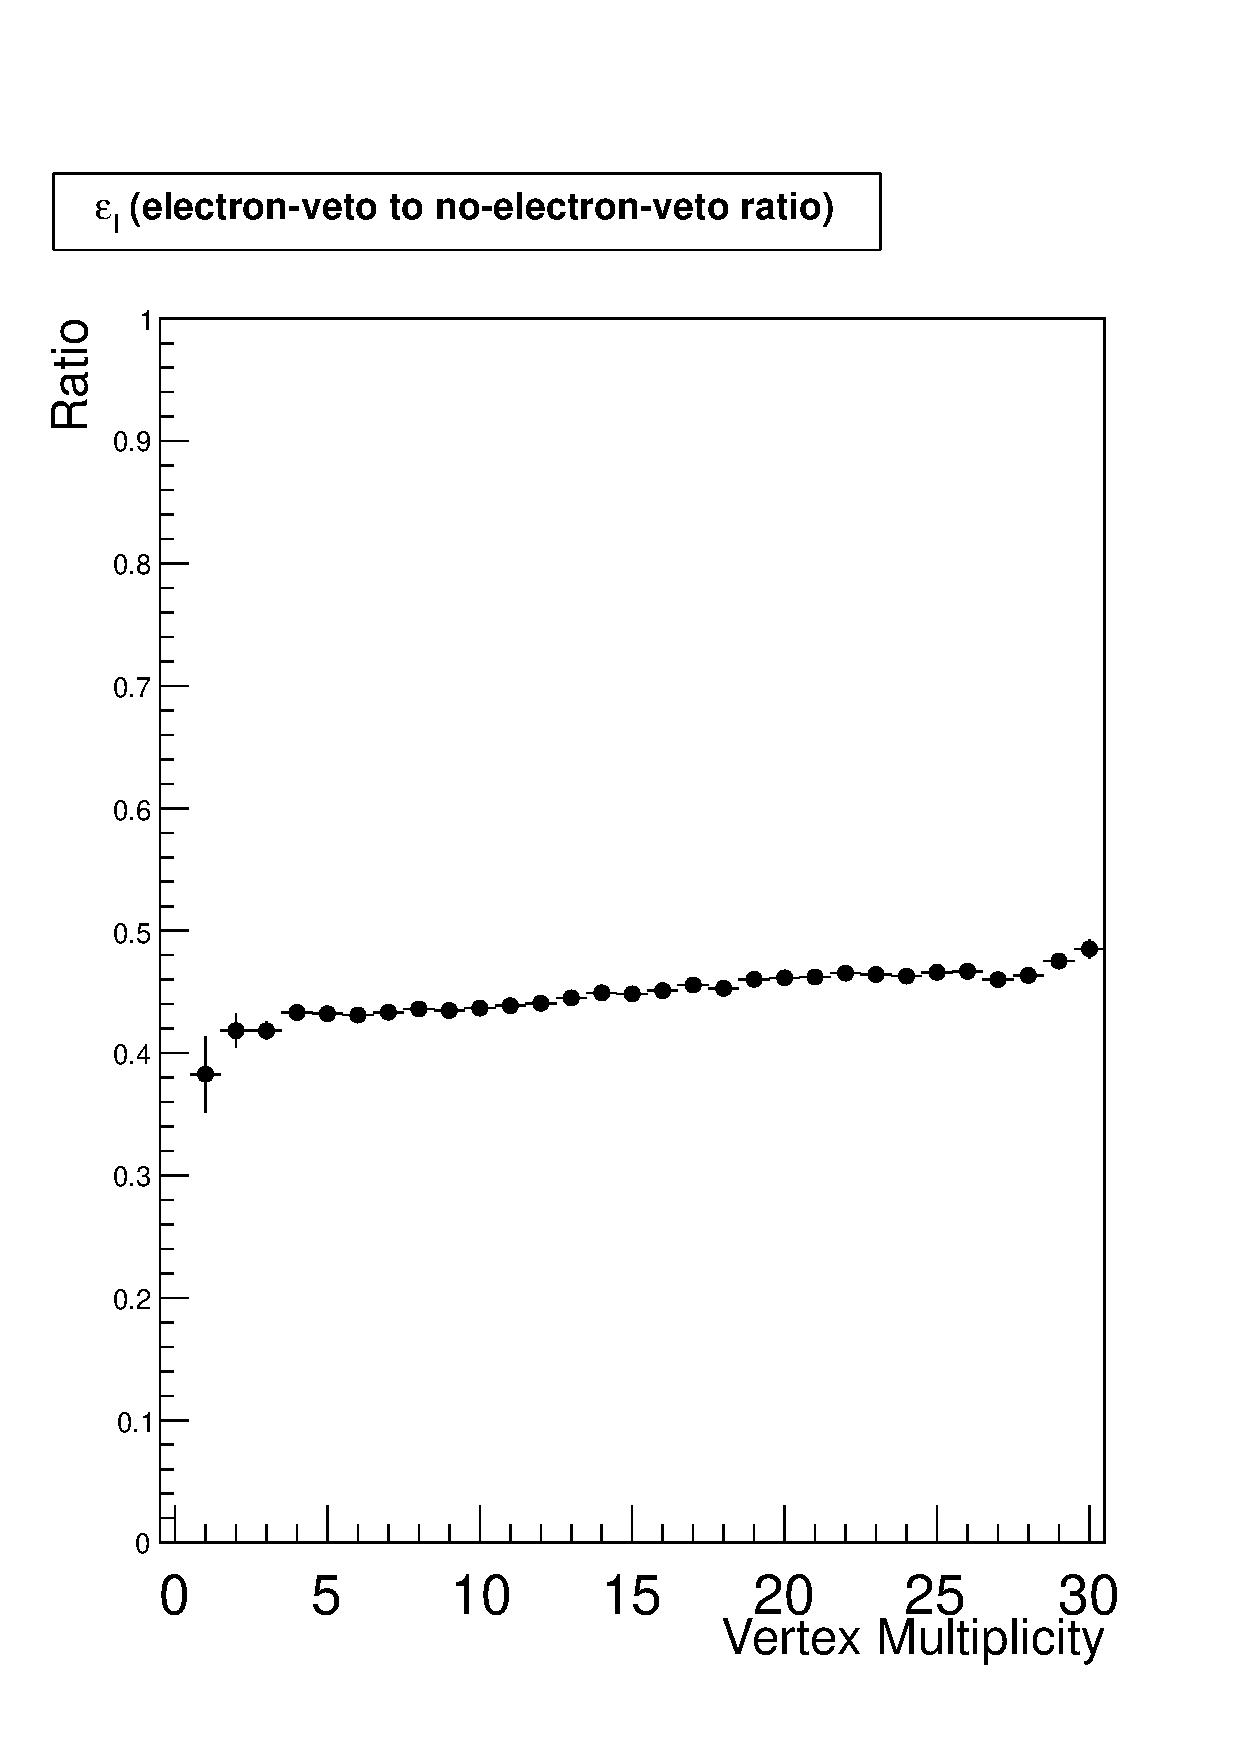
\includegraphics[width=0.8\textwidth]{FakeRateRatio_NVTX}
    \caption{\label{FNVTX} $\epsilon l$: electron-veto to no-electron-veto ratio to NVTX .}
\end{figure}

\begin{figure}[!hbt]
\centering
    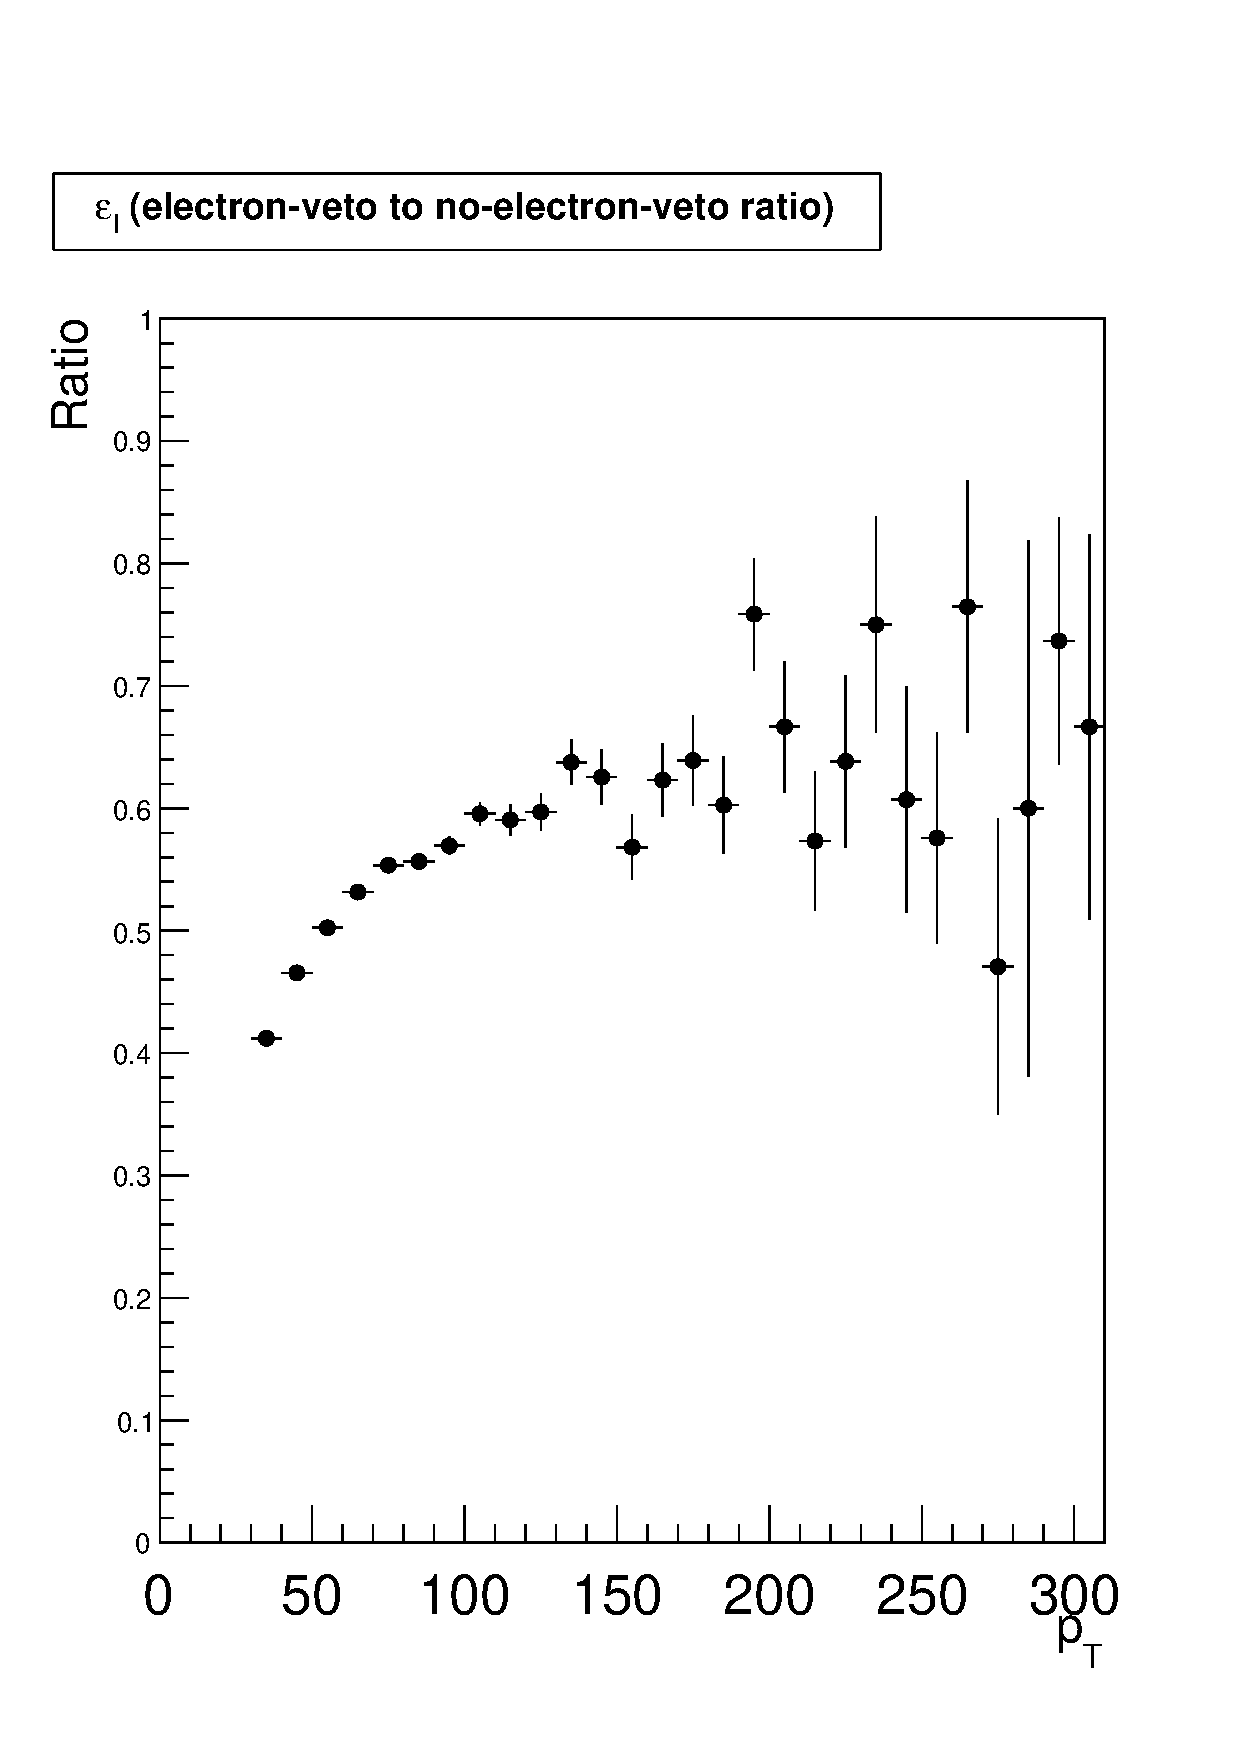
\includegraphics[width=0.8\textwidth]{FakeRateRatio_PT}
    \caption{\label{FPT} $\epsilon l$: electron-veto to no-electron-veto ratio to $P_T$ .}
\end{figure}

\textbf{Tag and Probe Method \cite{R23}:}  
Efficiencies can be calculated by using tag and probe which is data driven technique. a mass resonance (i.e. J/$\psi$, upsilon or Z), or a well known PDF is needed for this calculation. The Tag is a muon or electron that passed from a very tight selection criteria and therefore have a very low fake rate while the probe has looser criteria. Moreover, The Passing Probe has tighter criteria than the probe, but not tighter than the Tag.


\subsubsection{Photon Fake Rate from jets}

A template fitting technique is used to estimate  the contribution from fake photons from jets.
Defining a fakeable object is appropriate for  efficiency calculation within this method. The fakeable object is defined as an EM SuperCluster (SC) has certain characteristics:

\begin{itemize}

\item The SC has to be close to a jet within a $\Delta R$ distance of 0.5. This should reduce the real photon contamination.
\item The SC has to pass looser ID cuts, with respect to the tight ID selection. The ID cuts are loosened by a factor of 5.
\item The SC has to pass inverted tight ID cuts, for 1/5 of the H/E tower threshold, the charge isolation, the neutral isolation and the photon isolation cuts.

\end{itemize}

Once the FO is defined, the $\sigma_{i \eta i \eta}$ distribution of these objects can be fitted according to a template fit and obtain the signal fraction (which in this case will determine the number of fake photons from jets) and 
subtract the background component (which will be represented by the real photons). 

In order to perform the fit, the background and signal templates are obtained respectively from data and from MC corrected with data-driven correction factors. 

The corretions for the signal are the following:

\begin{eqnarray}
\label{ieta}
\sigma_{i \eta i \eta}^{EB corr} = (\sigma_{i \eta i \eta} - 0.0090405) \times 1.04 + 0.0089405 \nonumber \\
\sigma_{i \eta i \eta}^{EE corr} = \sigma_{i \eta i \eta} \times 1.1 - 0.0025 \nonumber \\
\end{eqnarray}

In Eq. \ref{ieta} , $\sigma_{i \eta i \eta}^{EB corr}$ is for the Barrel and $\sigma_{i \eta i \eta}^{EE corr}$ is for Endcap photons. Furthermore, the possible residual small differences between the true signal shapes and those used in the fit are taken into account by applying a systematic uncertainty on the shape while calculating the $\epsilon_{j}$s. 

The MC process used to infer the signal templates is the photon+jets, which has trasnverse momentum spectra reasonably similar to that of the all background processes. 

The background templates are taken directly from the data. The FO definition has been optimized to obtain a signal photon contamination fraction of less than 1$\%$. In addition to this it is veryfied that the background $\sigma_{i \eta 
i \eta}$ shape for the FO definition and the tight ID defintion are reasonably similar using the MC. However, any possible residual difference is taken into account from the shape systematic. 

After the shapes are obtained the Barrel and Endcap $\sigma_{i \eta i \eta}$ distribution separately can be fitted. The fit is performed on the entire $\sigma_{i \eta i \eta}$ range, but it is integrated over the tight ID $\sigma_{i \eta i \eta}$ range to obtain the number of events and the signal fraction. 

The results for photon fake rate from jets will be represented CMS Physics analysis note \cite{R34}. The final results for fake rate calculations are given in section \ref{fakerate}.

%%%%%%%%%%%%%%%%%%%%%%%%%%%%%%%%%%%%%%%%%%%%%%%%%%%%
\subsubsection{Photon Signal Efficiency}

In this case again a Tag and Prone technique is used as in the case of the fake rate from leptons. The $\epsilon_{s}$
is defined the per-object ratio of the photon efficiency for the tight selection over the sum of the efficiencies  for 
the no-electron-veto selection and the FO selection. However, the FO selection has been optimized to have negligible real photon contamination, therefore it will not be taken into account.

\begin{figure}[!ht]
  \begin{center}
       \resizebox{10cm}{!}{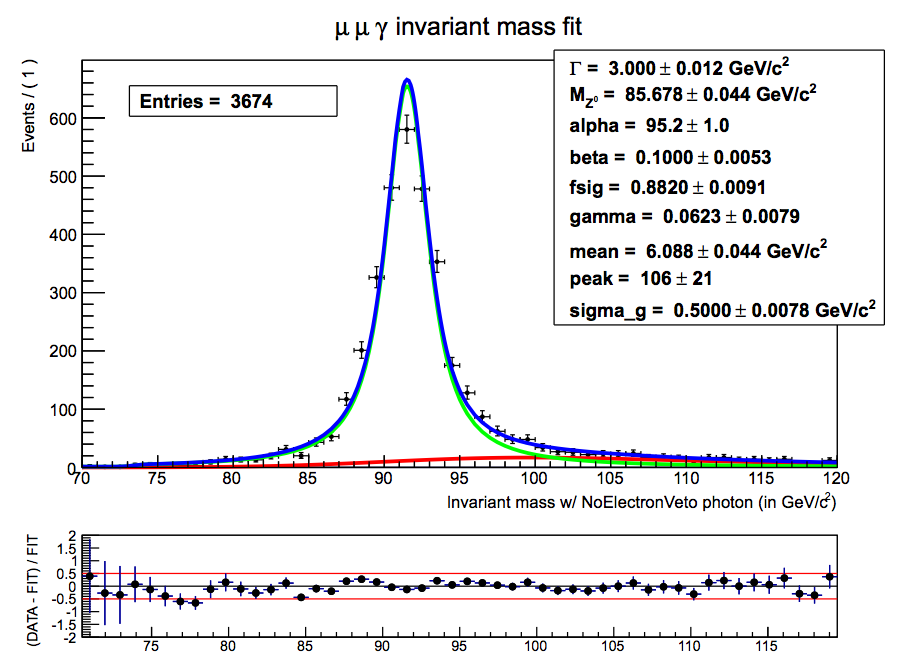
\includegraphics{Zmass_NoElectronVeto}} 
       \resizebox{10cm}{!}{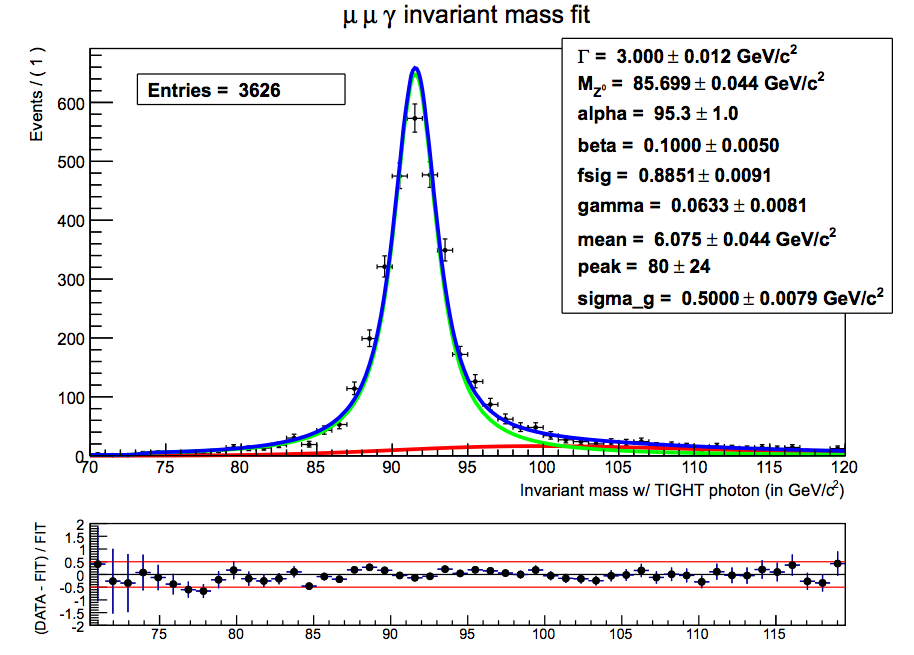
\includegraphics{Zmass_TIGHT}} 
  \end{center}
    \caption{Muon-Muon-Photon invariant mass fit for the no-electron-veto selection (upper plot) and the tight ID selection (lower plot). The fit fuction is a BreitWigner convoluted thanks to a fast Fourier trasformation to a 
Gaussian (for the signal) plus a CMSShape (for the background).}
    \label{Zmass_signal}
\end{figure}

In order to count the number of fake photons for the tight and no-electron-veto selection, Tag and Probe technique is applied on the invariant mass of the muon-muon-photon system. 

For the fit of the invariant mass a BreitWigner convoluted to a Gaussian (for the signal) with a fast Fourier trasformation plus a CMSShape for the Background. This allows to subtract the non Drell-Yan component. The final 
number of fitted signal events is the number of real photons to be used for the  $\epsilon_{s}$ calculation.

For the object selection for fake photon calculation, it is observed that the jet multiplicity has no effect on this calculation so no selection on the jet multiplicity is applied for the photon signal efficiency calculation. The transverse momentum of the photon is larger then 30 GeV/c. On the leading muon transverse momentum we apply a tight selection and we lower the transverse momenta criteria to 20 GeV in order to get enough statistics at the low end of the invariant mass distribution. 

Figure \ref{Zmass_signal} shows the fit performed in the invariant mass range between 70 and 120 GeV. Both DoubleMu and SingleMu Primary Datasets are used to increase statistics.

\subsubsection{Ratio Factors}

The ratio factors are determined from the data. To determined all the ratio factors is enough to determined the following number of events: $N^{sl}_{L}$, $N^{sq}_{L}$, $N^{sg}_{L}$, $N^{qg}_{L}$, $N^{lg}_{L}$, $N^{lq}_{L}$, 
$N^{ll}_{L}$, 
$N^{qq}_{L}$, $N^{gg}_{L}$. 

In a good approximation the above number of events can be obtained by selecting two photons events in which as $s$, $l$, $g$, $q$ photons, one can request a tight, anti-electron-veto, FO Quark-like and FO Gluon-like object, 
respectively. 
Any contamination due to this approximation can be subtracted by subtracting from MC the non-matching component (where in this case the matching is a MC matching to obtain true objects). 

Given the FO defition used the number of two photon-like object events containing at least one FO is small. In order to increase the statistics another FO defintion has been used. The alternative FO definition has been used to 
infer the ratio factors, after applying a correction factor which is derived from the data. The correction factor takes into account the ratio of the two FO definitions on a per-object base.  

\subsubsection{Results of Fake Rate Calculations}
\label{fakerate}

The $N^{ff}_{T}$ and $N^{sf}_{T}$ can be obtained by matrix inversion after the ratio factors, real photon efficiency and the fake rates are calculated. 10 Million pseudo-experiments are used in order to calculate the uncertainties and solutions with negative number of events are rejected. In the pseudo-experiments the ratio factors and the $\epsilon$s are allowed to alter within their uncertainties.

The final results are: $N_{sf}^{T} =  7.9 \pm 0.4$ and $N_{ff}^{T} =  1.7  \pm 0.08$.


%%%%%%%%%%%%%%%%%%%%%%%%%%%%%%%%%%%%%%%%%%%%%%%%%%%%%%%%%%%%
%%%%%%%%%%%%%%%%%%%%%%%%%%%%%%%%%%%%%%%%%%%%%%%%%%%%%%%%%%%%
\chapter{CONCLUSION}

Pair produced excited quark, $t^*$, which decays exclusively to a top quark and a photon, is investigated by considering semi-leptonic decay channel. In final state, there are two isolated photons, at least 4 well-reconstructed jets and one lepton, which can be either a single isolated muon or electron. Furthermore, the $\chi ^2$  sorting method and matrix method is presented to reconstruct signal and to determine fake rate of photons coming from leptons and jets, respectively. Tag and Probe method and QCD-enriched samples are also implied to make use of matrix method. In this study, proton-proton collision data collected by CMS at 8 TeV corresponding to an integrated luminosity of 19.6${fb}^{-1}$ is investigated. Analysis is performed in a model independent way while a heavy spin-3/2 excitation of a heavy spin-1/2 quark indicated by ”Rarita-Schwinger” vector spinor Lagrangian is the most favourable choice among other beyond the standard models. As a result of this study, no significant excess is observed over expectations and a lower limit is set on a $t^*$  quark mass of 969 ${GeV/c}^{2}$ at 95$\%$ confidence level. Limit calculations are performed using Asymptotic CLs method \cite{R22} with Poisson statistics. A log-normal prior is used in the integration given the background uncertainty. Figure \ref{SignalCl} shows the crossection of $t^*$  while x axis is mass. 

\begin{figure}[!hbt]
\centering
    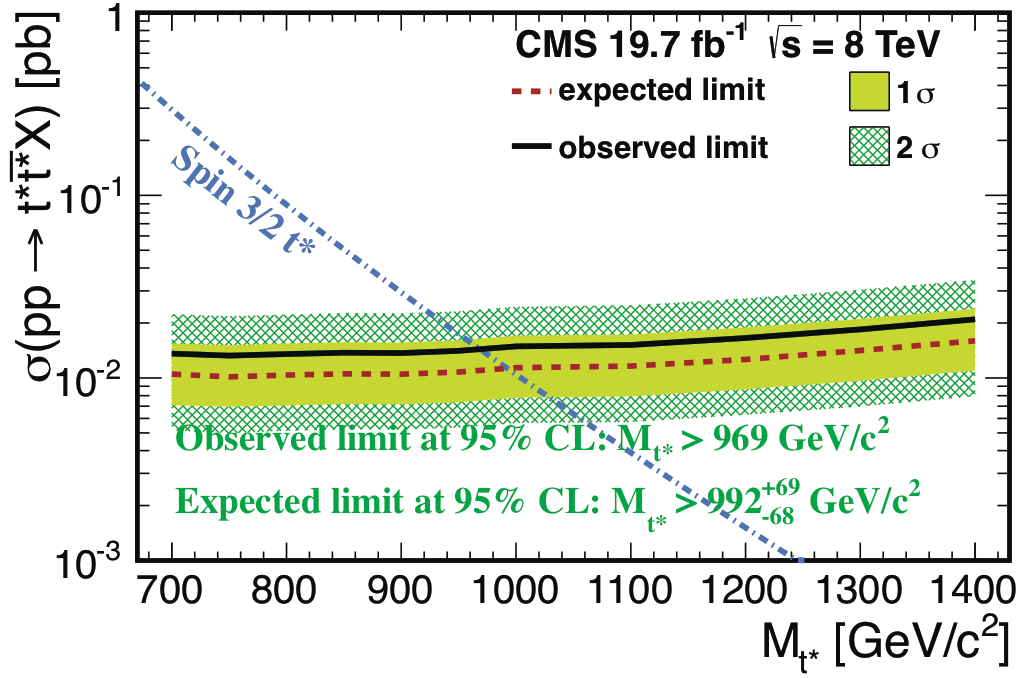
\includegraphics[width=0.8\textwidth]{SignalCl}
    \caption{\label{SignalCl} the crosection of t* while x axis is mass.}
\end{figure}


%%%%%%%%%%%%%%%%%%%%%%%%%%%%%%%%%%%%%%%%%%%%%%%%%%%%%%%%%%%%
%
% References in Bibtex format goes into below indicated file with .bib extension
%%%\bibliography{thesis_references}
% You can use full name of authors, however most likely some of the Bibtex entries you will find, will use abbreviated first names
% If you don't want to correct each of them by hand, you can use abbreviated style for all of the references
%%%\bibliographystyle{abbrv}



%%%%%%%%%%%%%%%%%%%%%%%%%%%%%%%%%%%%%%%%%%%%%%%%%%%%%%%%%%%%
%%%%%%%%%%%%%%%%%%%%%%%%%%%%%%%%%%%%%%%%%%%%%%%%%%%%%%%%%%%%

%%%%%%%%%%%%%%%%%%%%%%%%%%%%%%%%%%%%%%%%%%%%%%%%%%%%%%%%%%%%
%%%%%%%%%%%%%%%%%%%%%%%%%%%%%%%%%%%%%%%%%%%%%%%%%%%%%%%%%%%%
%%\appendix
%%\chapter{Matrix method}

%%%%This is appendix text.
%
% If you are a Ph.D. Student you need to insert a CV at the end of you thesis
% Check vita.tex for a simple CV template in Latex

\begin{thebibliography}{99}\fontsize{12}{16.4} \selectfont

\bibitem{R24}	J. Beringer et al. (Particle Data Group), PR D86, 010001 (2012) \url{http://pdg.lbl.gov} , last visited 09/07/2014

\bibitem{R25}	H. Georgi, L. Kaplan, D. Morin, and A. Schenk, “Effects of top compositeness”, Phys.Rev. D51 (1995) 3888–3894, doi:10.1103/PhysRevD.51.3888, arXiv:hep-ph/9410307, last visited 09/07/2014.

\bibitem{R26}	E. Eichten, K. D. Lane, and M. E. Peskin, “New Tests for Quark and Lepton Substructure”, Phys.Rev.Lett. 50 (1983) 811–814, doi:10.1103/PhysRevLett.50.811.

\bibitem{R12}	D. A. Dicus, S. Gibbons, and S. Nandi, “Collider production of spin 3/2 quarks”, \url{arXiv:hep-ph/9806312}.

\bibitem{R27}	B. Lillie, J. Shu, and T. M. Tait, “Top Compositeness at the Tevatron and LHC”, JHEP 0804 (2008) 087, doi:10.1088/1126-6708/2008/04/087, arXiv:0712.3057.

\bibitem{R28}	A. Pomarol and J. Serra, “Top Quark Compositeness: Feasibility and Implications”, Phys.Rev. D78 (2008) 074026, doi:10.1103/PhysRevD.78.074026, arXiv:0806.3247.

\bibitem{R29}	K. Kumar, T. M. Tait, and R. Vega-Morales, “Manifestations of Top Compositeness at Colliders”, JHEP 0905 (2009) 022, doi:10.1088/1126-6708/2009/05/022, arXiv:0901.3808.

\bibitem{R30}	L. Randall and R. Sundrum, “A Large mass hierarchy from a small extra dimension”, Phys.Rev.Lett. 83 (1999) 3370–3373, doi:10.1103/PhysRevLett.83.3370, arXiv:hep-ph/9905221.

\bibitem{R31}	L. Randall and R. Sundrum, “An Alternative to compactification”, Phys.Rev.Lett. 83 (1999) 4690–4693, doi:10.1103/PhysRevLett.83.4690, arXiv:hep-th/9906064.

\bibitem{R9}	Schmaltz, M. (2002). Physics beyond the standard model (theory): Introducing the little higgs. ICHEP 2002.

\bibitem{R32}	Griffiths, D. J. Introduction to Elementary Particles (New York, USA: Wiley, 1987).

\bibitem{RSM1}	CMS Collaboration, “Observation of a new boson at a mass of 125 GeV with the CMS experiment at the LHC”, Phys. Lett. B 716 (2012), no. 1, 30 - 61, doi:10.1016/j.physletb.2012.08.021.

\bibitem{RSM2}	ATLAS Collaboration, “Observation of a new particle in the search for the Standard Model Higgs boson with the ATLAS detector at the LHC”, Phys. Lett. B 716 (2012), no. 1, 1 - 29, doi:10.1016/j.physletb.2012.08.020.

\bibitem{SM}  Particle Data Group Collaboration, “Review of Particle Physics”, Phys. Rev. D 86 (2012) 010001, doi:10.1103/PhysRevD.86.010001.

\bibitem{R6}	Cacciapaglia, G., Deandrea, A., Harada, D., and Okada, Y. (2010). Bounds and decays of new heavy vector-like top partners. JHEP, Retrieved from \url{http://link.springer.com/article/10.1007} , last visited 09/07/2014


\bibitem{R7}	Hassanain, B., March-Russell, J., and Rosa, J. G. (2009). On the possibility of light string resonances at the lhc and tevatron from randall-sundrum throats. JHEP, Retrieved from \url{http://arxiv.org/abs/0904.4108} , last visited 09/07/2014

\bibitem{R33}	T. Kaluza, Sitzungsber. Preuss. Akad. Wiss. Berlin (Math. Phys.) K1, 966 (1921); O. Klein, Z. Phys. 37, 895 (1926).

\bibitem{R10}	Physics searches at the LHC. \url{arXiv: 0912.3259} [hep-ph] 4 Sep 2010.

\bibitem{R13}	W. Rarita and J. Schwinger, “On a theory of particles with half integral spin”, Phys.Rev. 60 (1941) 61, doi:10.1103/PhysRev.60.61.

\bibitem{R11}	B. Moussallam and V. Soni, “PRODUCTION OF HEAVY SPIN 3/2 FERMIONS IN COLLIDERS”, Phys.Rev. D39 (1989) 1883–1891, doi:10.1103/PhysRevD.39.1883.

\bibitem{R1}	CERN, “CERN faq LHC the guide.” \url{http://cds.cern.ch/record/1165534/files/CERN-Brochure-2009-003-Eng.pdf} , last visited 09/07/2014

\bibitem{R2}	CERN,”CMS.” \url{http://cms.web.cern.ch/news/cms-detector-design}, last visited 09/07/2014

\bibitem{R3}	The CMS Collaboration, “The CMS experiment at the CERN LHC,” Journal of Instrumentation, vol. 3, 2008. 2.2 [JINST 3 S08004]

\bibitem{R15}	\url{http://www.hephy.at/user/friedl/diss/html/node26.html} , last visited 09/07/2014

\bibitem{R16}	The CMS Collaboration, “The CMS experiment at the CERN LHC”, Journal of Instrumentation, Vol. 3, No. 08, pp. S08004, 2008

\bibitem{R17}	The CMS Collaboration,"Technical Design Report of HCAL" \url{https://cds.cern.ch/record/357153/files/CMS_HCAL_TDR.pdf}, last visited 09/07/2014

\bibitem{R18}	The CMS Collaboration,"Offline Workbook" \url{https://twiki.cern.ch/twiki/bin/view/CMSPublic/WorkBookChapter3}, last visited 09/07/2014

\bibitem{Mad}	F. Maltoni and T. Stelzer, “MadEvent: Automatic event generation with MadGraph”, JHEP 0302 (2003) 027, arXiv:hep-ph/0208156.

\bibitem{Cteq}	J. Pumplin et al., “New generation of parton distributions with uncertainties from global QCD analysis”, JHEP 0207 (2002) 012, arXiv:hep-ph/0201195.

\bibitem{Pythia}	T.Sjostrand, S.Mrenna, and P.Z.Skands, “PYTHIA 6.4 Physics and Manual”, JHEP 0605 (2006) 026, doi:10.1088/1126-6708/2006/05/026, arXiv:hep-ph/0603175.

\bibitem{Geant}	J. Allison et al., “Geant4 developments and applications”, IEEE Trans.Nucl.Sci. 53 (2006)
270, doi:10.1109/TNS.2006.869826.

\bibitem{PF1}	CMS Collaboration, “Particle-Flow Event Reconstruction in CMS andPerformance for Jets, Taus, and MET”, CMS-PAS PFT-09-001 (2009).

\bibitem{PF2}	CMS Collaboration, “Commissioning of the Particle Flow reconstruction in Minimum Bias and Jet Events from pp Collisions at 7 TeV”, CMS-PAS PFT-10-002 (2010).

\bibitem{PF3}	CMS Collaboration, “Commissioning of the Particle flow Event Reconstruction with the first LHC collisions recorded in the CMS detector”, CMS Physics Analysis Summary CMS PAS PFT 10 001, CERN, (2010).

\bibitem{PF4}	CMS Collaboration, “Commissioning of the particle flow event reconstruction with leptons from J/Y and W decays at 7 TeV”, CMS Physics Analysis Summary CMS-PAS-PFT-10-003, CERN, (2010).

\bibitem{trigger}	CMS Collaboration, \url{https://hypernews.cern.ch/HyperNews/CMS/get/top/1602.html} , last visited 09/07/2014

\bibitem{R21}	CMS Physics Object Group, “Baseline muon selection” \url{https://twiki.cern.ch/twiki/bin/view/CMSPublic/SWGuideMuonId} , last visited 09/07/2014

\bibitem{electron}	CMS Physics Object Group, "EgammaCutBasedIdentification",  \url{https//twiki.cern.ch/twiki/bin/view/CMS/EgammaCutBasedIdentification} , last visited 09/07/2014

\bibitem{photon}	 CMS Physics Object Group, "PhotonID 2012" \url{https://twiki.cern.ch/twiki/bin/view/CMS/CutBasedPhotonID2012} , last visited 09/07/2014

\bibitem{jet} CMS JetMet Group, "Jet ID", \url{https://twiki.cern.ch/twiki/bin/viewauth/CMS/JetID} , last visited 09/07/2014

\bibitem{antikt} Cacciari, M., Salam, G., P. and Soyez, G., “The anti-kt jet clustering algorithm”, Journal of High Energy Physics, Vol. 2008, No. 04, pp. 063, 2008.

\bibitem{pileup}	CMS Collaboration, \url{https://twiki.cern.ch/twiki/bin/view/CMS/Pileup_MC_Gen_Scenarios# 2012_Pileup_Scenario_s} , last visited 09/07/2014

\bibitem{R35}	Babar Collaboration, "A User’s Guide to the RooFitTools Package for Unbinned Maximum Likelihood Fitting", 2001, \url{http://webcms.ba.infn.it/cms-software/RooFit/RooFitToolsManual.pdf} , last visited 09/07/2014


\bibitem{R23}	N. Adam et. al., "Tag and Probe Tutorial CMSSW 3 1 2", 2001.

\bibitem{R34}	E. Asilar Y. Chang, M. Cardaci, K. Chen, M. Guler, Y. Tzeng, and S. Yu, "Search for an excited quark decaying to a top quark plus photon", CMS AN-2014/030.


\bibitem{R22}	G. Cowan, K. Cranmer, E. Gross, and O. Vitells, "Asymptotic formulae for likelihood-based tests of new physics", The European Physical Journal C 71 (2011), no. 2,1–19, doi:10.1140/epjc/s10052-011-1554-0, arXiv:1007.1727.




\end{thebibliography}


%\curriculumvitae
\label{chapter:vita}

\section*{\uppercase{Personal Information}}

\textbf{Surname, Name: } Surname, Name\\
\textbf{Nationality:} Turkish (TC) \\
\textbf{Date and Place of Birth:} Birthday, Birthplace\\
\textbf{Marital Status:} Marital Status \\
\textbf{Phone:} Phone Number \\
\textbf{Fax:} Fax Number \\

\section*{\uppercase{Education}}

\begin{tabular}{lll}
\textbf{Degree} & \textbf{Institution} & \textbf{Year of Graduation} \\
M.S. & M.S. Institute & M.S. Year \\
B.S. & B.S. Institute & B.S. Year \\
High School & High School Name & High School Graduating Year
\end{tabular}

\section*{\uppercase{Professional Experience}}

\begin{tabular}{lll}
\textbf{Year} & \textbf{Place} & \textbf{Enrollment} \\
Duration 1 & Institute/Company 1 & Role/Position/Experience 1 \\
Duration 2 & Institute/Company 2 & Role/Position/Experience 2 
\end{tabular}

\section*{\uppercase{Publications}}
\subsection*{International Conference Publications}
Your publications goes here. Do not try to use Bibtex, since Bibtex builds a single bibliography
database for the document.

\end{document}
